%!TEX root = ../main.tex
\chapter{Methodology}
Reverse engineering is a complex process with no universal solution. It often involves extensive trial and error, making it important to adopt a strategy that encourages rapid iteration while minimizing risk. In this case, the most practical approach was to prioritize simplicity and accessibility. The Android version of the app was selected for analysis, as it uses Java and Kotlin—languages that are generally more amenable to reverse engineering. Additionally, a man-in-the-middle (MITM) technique was chosen to intercept and manipulate data exchanged between the app and the target device.

The initial step involved verifying the ability to interact with the app by modifying data in a detectable way. Once this was confirmed, the next objective was to capture the data being transmitted between the app and the makeup printing device, along with identifying the method of transmission. The final step was to replicate that communication in order to send custom data to the device in the expected format.

\section{Decoding app data}
When trying to understand the communications between the app and the makeup printer device, one method that’s certifiably free of interpretation error is capturing the packet data sent over the air between the devices. Understanding the raw packets is also helpful if the app itself is too difficult to reverse engineer, as it enables direct interaction with the device and bypasses the app altogether. This is a common reverse engineering method because developers seldom bother to obfuscate Bluetooth packet data. Ultimately, the relevant data has to appear somewhere in the Bluetooth packets, it’s just a matter of decoding where and how it does.

\subsection{Testing with the nRF Connect App}
There are a few different ways to capture this packet data. As mentioned previously, one method is using a Bluetooth packet sniffer along with the nRF Connect app and Wireshark. This was my first test. The following figures show the device information I discovered using the nRF Connect app. It was fascinating to see how much information was accessible through nRF Connect alone. For example, Figure \ref{fig:nrfconnect3} shows the NUS\_ID, NUS\_RX, and NUS\_TX identifiers, which I previously found in Jadx after a long period of searching. The nRF Connect app revealed this information immediately, without even needing to connect to the device.
\begin{figure}[H]
	\centering
	\begin{minipage}{0.32\textwidth}
		\centering
		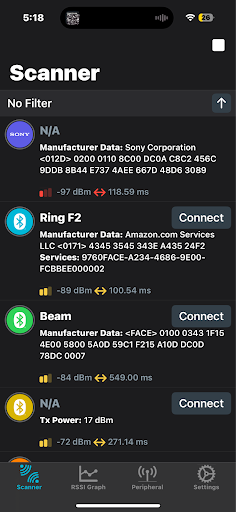
\includegraphics[width=0.8\linewidth]{nrfconnect1}
		\caption{nRF Connect Scanner page}
		\label{fig:nrfconnect1}
	\end{minipage}
	\hfill
	\begin{minipage}{0.32\textwidth}
		\centering
		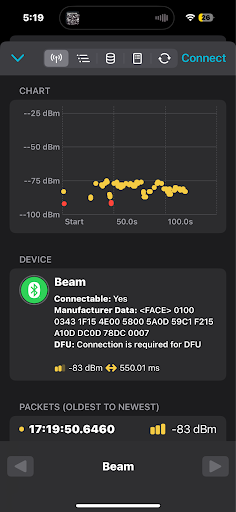
\includegraphics[width=0.8\linewidth]{nrfconnect2}
		\caption{nRF Connect Beam Beacon page}
		\label{fig:nrfconnect2}
	\end{minipage}
	\hfill
	\begin{minipage}{0.32\textwidth}
		\centering
		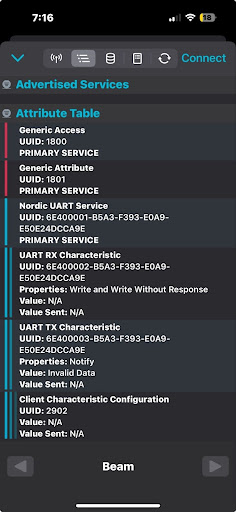
\includegraphics[width=0.8\linewidth]{nrfconnect3}
		\caption{nRF Connect Beam Services and Characteristics}
		\label{fig:nrfconnect3}
	\end{minipage}
	
	\caption{NRF Connect screenshots}
	\label{fig:nrfconnect_all}
\end{figure}

% TODO: \usepackage{graphicx} required
\begin{figure}[H]
	\centering
	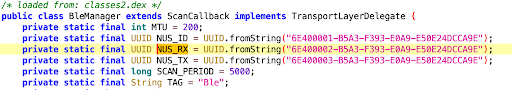
\includegraphics[scale=.8]{bleuuidjadx}
	\caption{Jadx App Gatt Profile Information}
	\label{fig:bleuuidjadx}
\end{figure}
Unfortunately, while this information was helpful, I wasn’t able to gather much more from nRF Connect because the device would connect and then disconnect shortly afterward. Even so, this discovery was valuable because it suggests that a handshake occurs between the app and device after connecting, which the nRF Connect app does not perform.

Without dumping the firmware, I cannot know exactly what occurs during this handshake. However, I can begin piecing it together by examining the onConnectionStateChanged() function in Jadx. Figure \ref*{fig:statemachineonconnection} presents a model of this function. It illustrates how the function checks Android’s BluetoothProfiles to determine whether the constant indicates a disconnected state (0) or a connected state (2). If connected, the function proceeds to request an MTU of 200 from the device. This is likely the point at which issues arise, as the app’s custom MTU is significantly larger than the general Bluetooth MTU used by the nRF Connect app.

% TODO: \usepackage{graphicx} required
\begin{figure}[H]
	\centering
	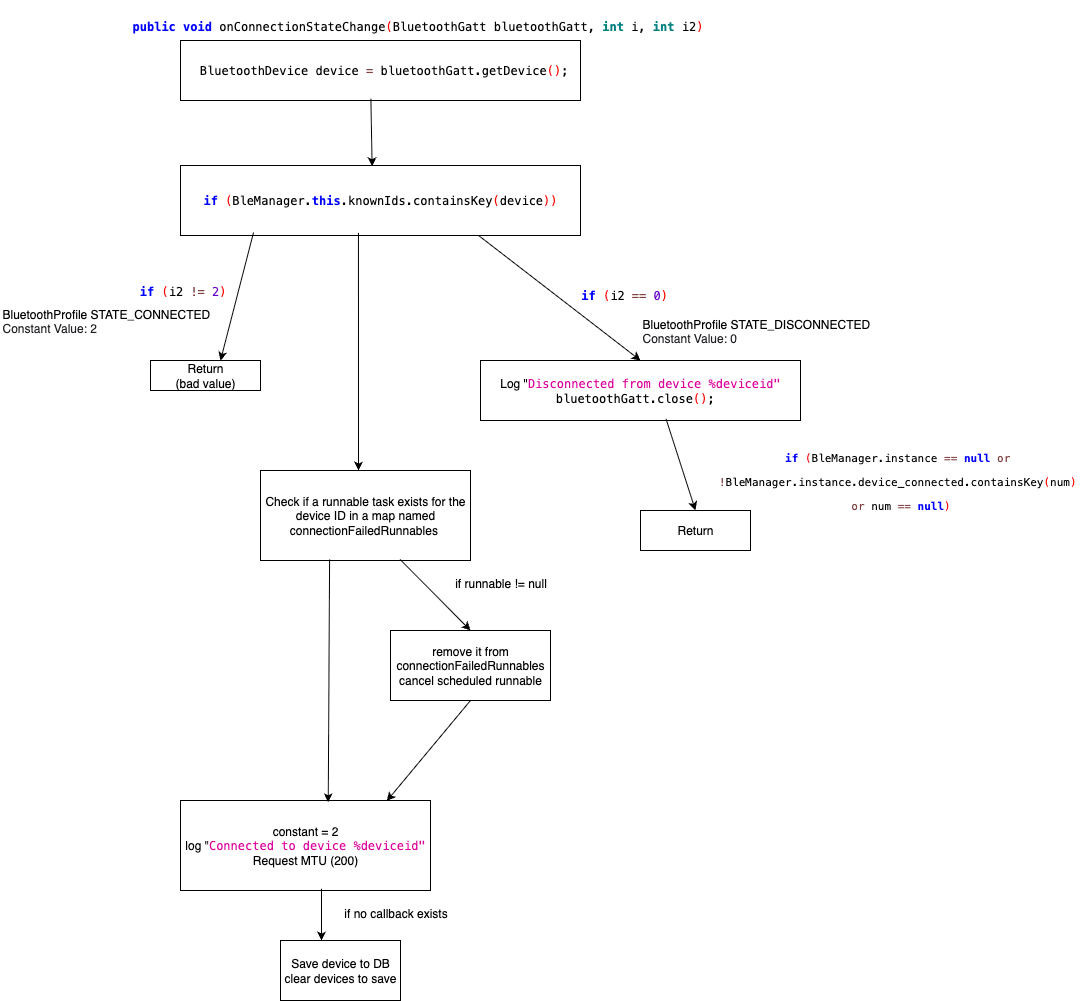
\includegraphics[scale=.5]{statemachineonconnection}
	\caption{onConnectionStateChange() State Machine}
	\label{fig:statemachineonconnection}
\end{figure}

Nevertheless, if the device had remained connected, it would have been possible to conduct tests and observe the raw byte payloads along with the characteristics transmitting them. For certain devices, it is even feasible to reverse engineer them using only the nRF Connect app, which is both impressive and somewhat concerning.


After discovering the connectivity issue on ios with the nrf app, I was able to access the device through the nRF Connect app by switching to Android. I had the nRF Connect app running when I opened the YSL app and connected to the device, which triggered a popup on my phone indicating that an “unknown device was detected” and asking whether I wanted to connect for debugging. 

When I reopened the nRF Connect app, the device and all of its packet information became visible. However, when I returned to the YSL app, the device appeared as disconnected and required me to disconnect it in the nRF Connect app before I could reestablish connectivity.
Using this workaround, I was able to run several tests and capture definitive live packet data. During these tests, the nRF Connect app attempted to translate the packet data into Unicode strings. This translation revealed that the shade information is transmitted by the device in one of the initial packets, regardless of whether a dispense occurs or a color is selected.
% TODO: \usepackage{graphicx} required
\begin{figure}[H]
	\centering
	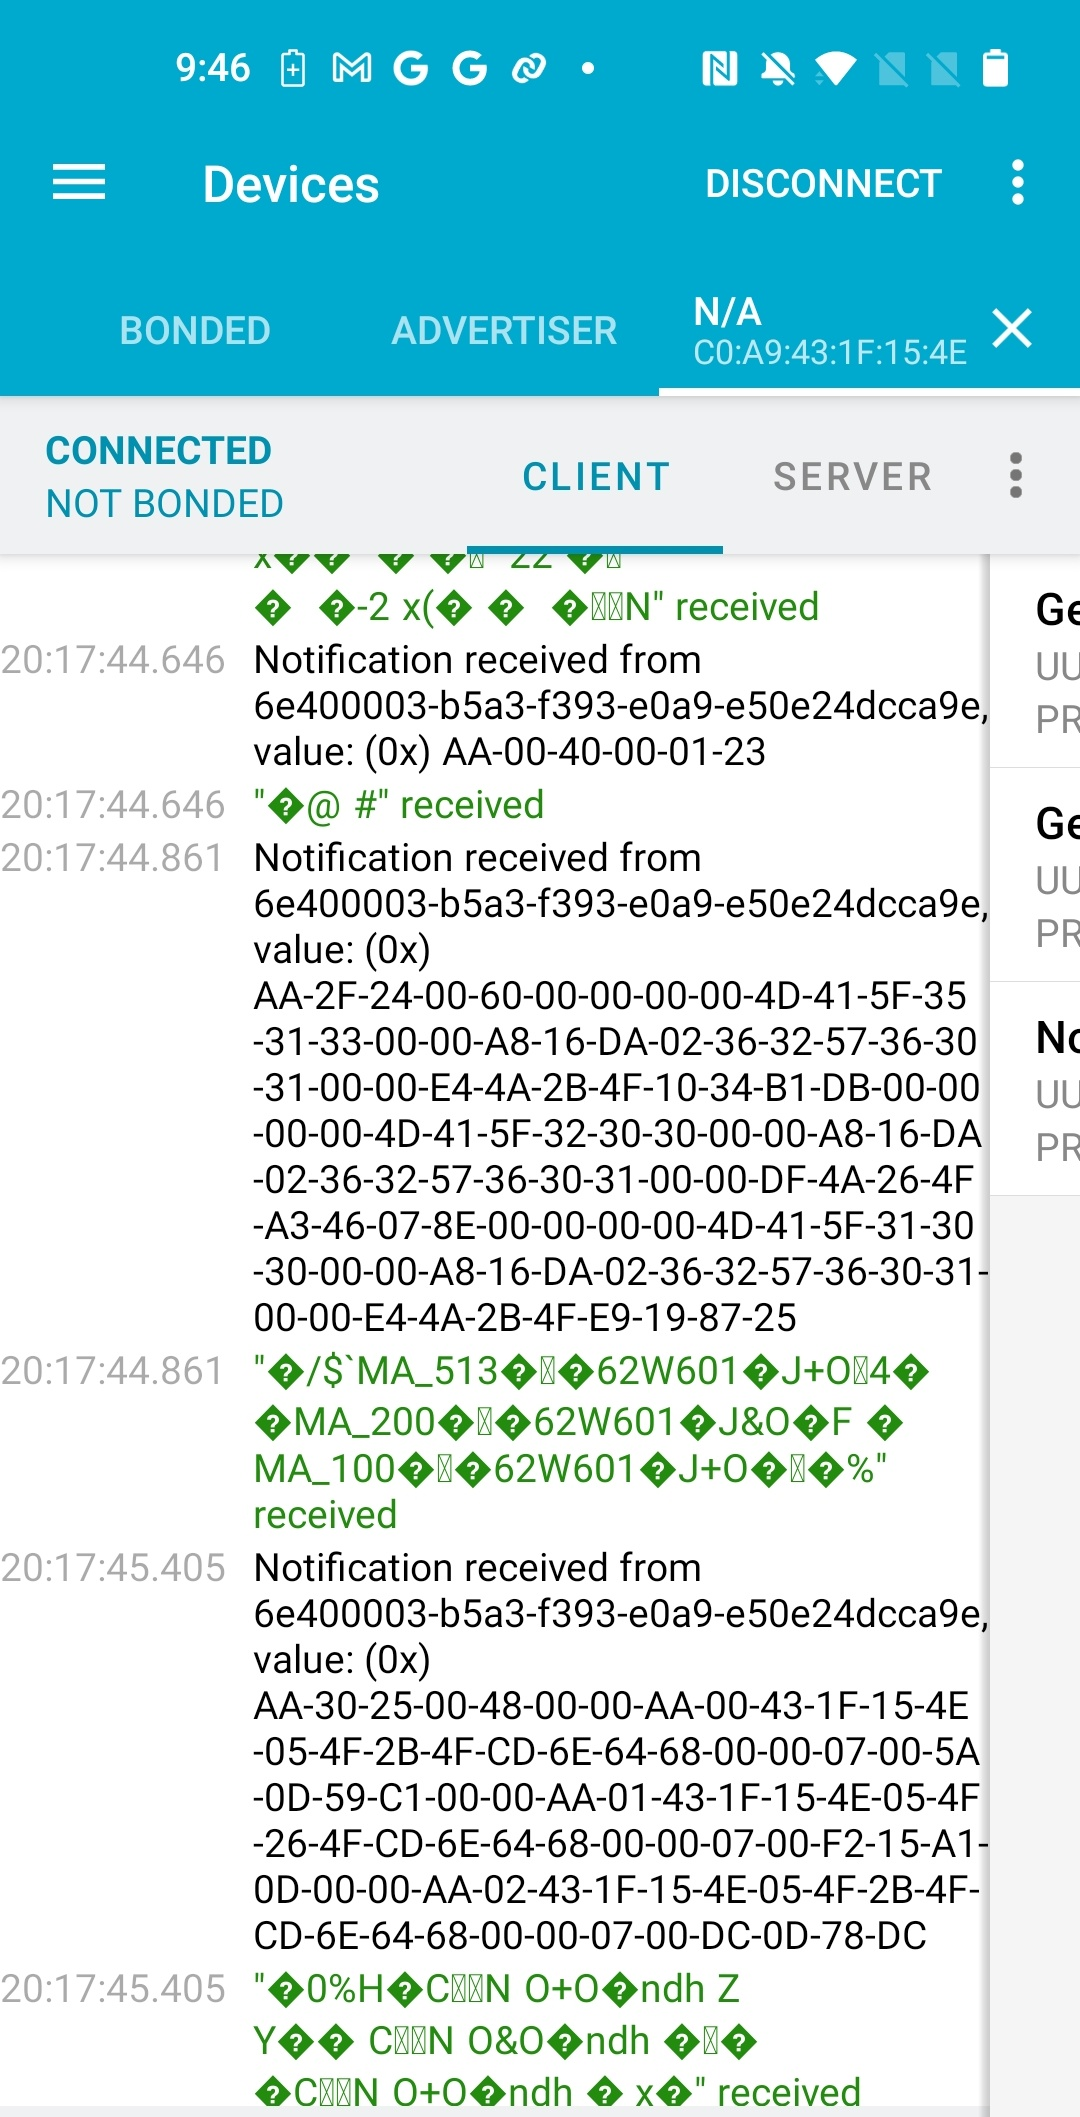
\includegraphics[scale=.145]{nrf_connect_android}
	\caption{nRF Connect Android Device Communication}
	\label{fig:nrfconnectandroid}
\end{figure}

\section{Testing with the nRF Sniffer and Wireshark}

In addition to using the nRF Connect app, a Bluetooth sniffer proved to be especially useful. While nRF Connect can capture communications received from the target device, it doesn’t show all Bluetooth traffic. Bluetooth sniffers, on the other hand, can capture the full set of Bluetooth commands exchanged between devices. The main drawback of relying solely on a sniffer is the lack of built-in packet decoding or interpretation. Using both tools together offers the most complete picture of the communication.

When selecting a sniffer, I had to weigh the overall cost of setting up the environment, which led me to choose the nRF52840 Dongle. My research indicated that this dongle was reliable and offered significant value for its modest \$10 cost. Additionally, it is manufactured by the same company that appeared to provide the software development kit used by the target device. Although more advanced and expensive sniffers can yield more detailed results, I recommend that anyone beginning this process start with a reasonably priced sniffer and consider investing in a higher-end tool only if the initial setup proves insufficient.

Setting up the nRF52840 Dongle required several steps. The dongle itself is simply a piece of hardware that serves no specific function until the appropriate software is flashed onto it. The first step involved installing the nRF Util tool, which depends on the presence of the SEGGER J-Link software. If this software is missing, outdated, or incorrectly configured in the system path, the flashing process will not work properly. The next requirement was to install the ble-sniffer command. Completing these installations prepared the environment for flashing the dongle.

The subsequent step involved locating the directory where nRF Util was installed. Within this directory, the corresponding firmware for the sniffer could be found, usually named in the format sniffer\_nrf52840dongle\_nrf52840\_*.zip. After connecting the dongle to my computer—I use a MacBook equipped only with USB-C ports, though a USB adapter functioned without issue—I proceeded to install the nRF Util device command using nrfutil install device. Running the command nrfutil device list allowed me to identify the correct device. Once detected, I programmed the dongle by executing nrfutil device program with the options \textbf{\texttt{--serial-number <serial-number> --firmware <file>}}, substituting the serial number identified earlier and the appropriate firmware file. At this stage, the dongle was flashed and ready for use.

Following these steps, I was able to begin sniffing Bluetooth traffic immediately. When the dongle successfully captured packets, an LED light on the device would blink with each sniffed packet. The setup functioned perfectly on the first day. However, during retesting the following day, the LED stopped blinking, and the dongle was not recognized correctly. Diagnosing the problem required extensive troubleshooting. Sometimes, the dongle appeared in the nRF Connect app, while at other times it disappeared entirely and was not visible from the command line. Ultimately, I had to wipe the dongle and repeat the flashing process, which seemed to restore its functionality.

Nevertheless, I encountered a significant issue: the dongle worked a bit too well. I was testing in a densely populated apartment complex where numerous Bluetooth devices were active, as previously observed through the nRF Connect app. The dongle’s LED blinked incessantly, making it impossible to isolate packets relevant only to my target device and specific tests. Figure \ref{fig:wiresharkpacketsniffing} illustrates a log in which the dongle captured over 32,400 packets.

% TODO: \usepackage{graphicx} required
\begin{figure}
	\centering
	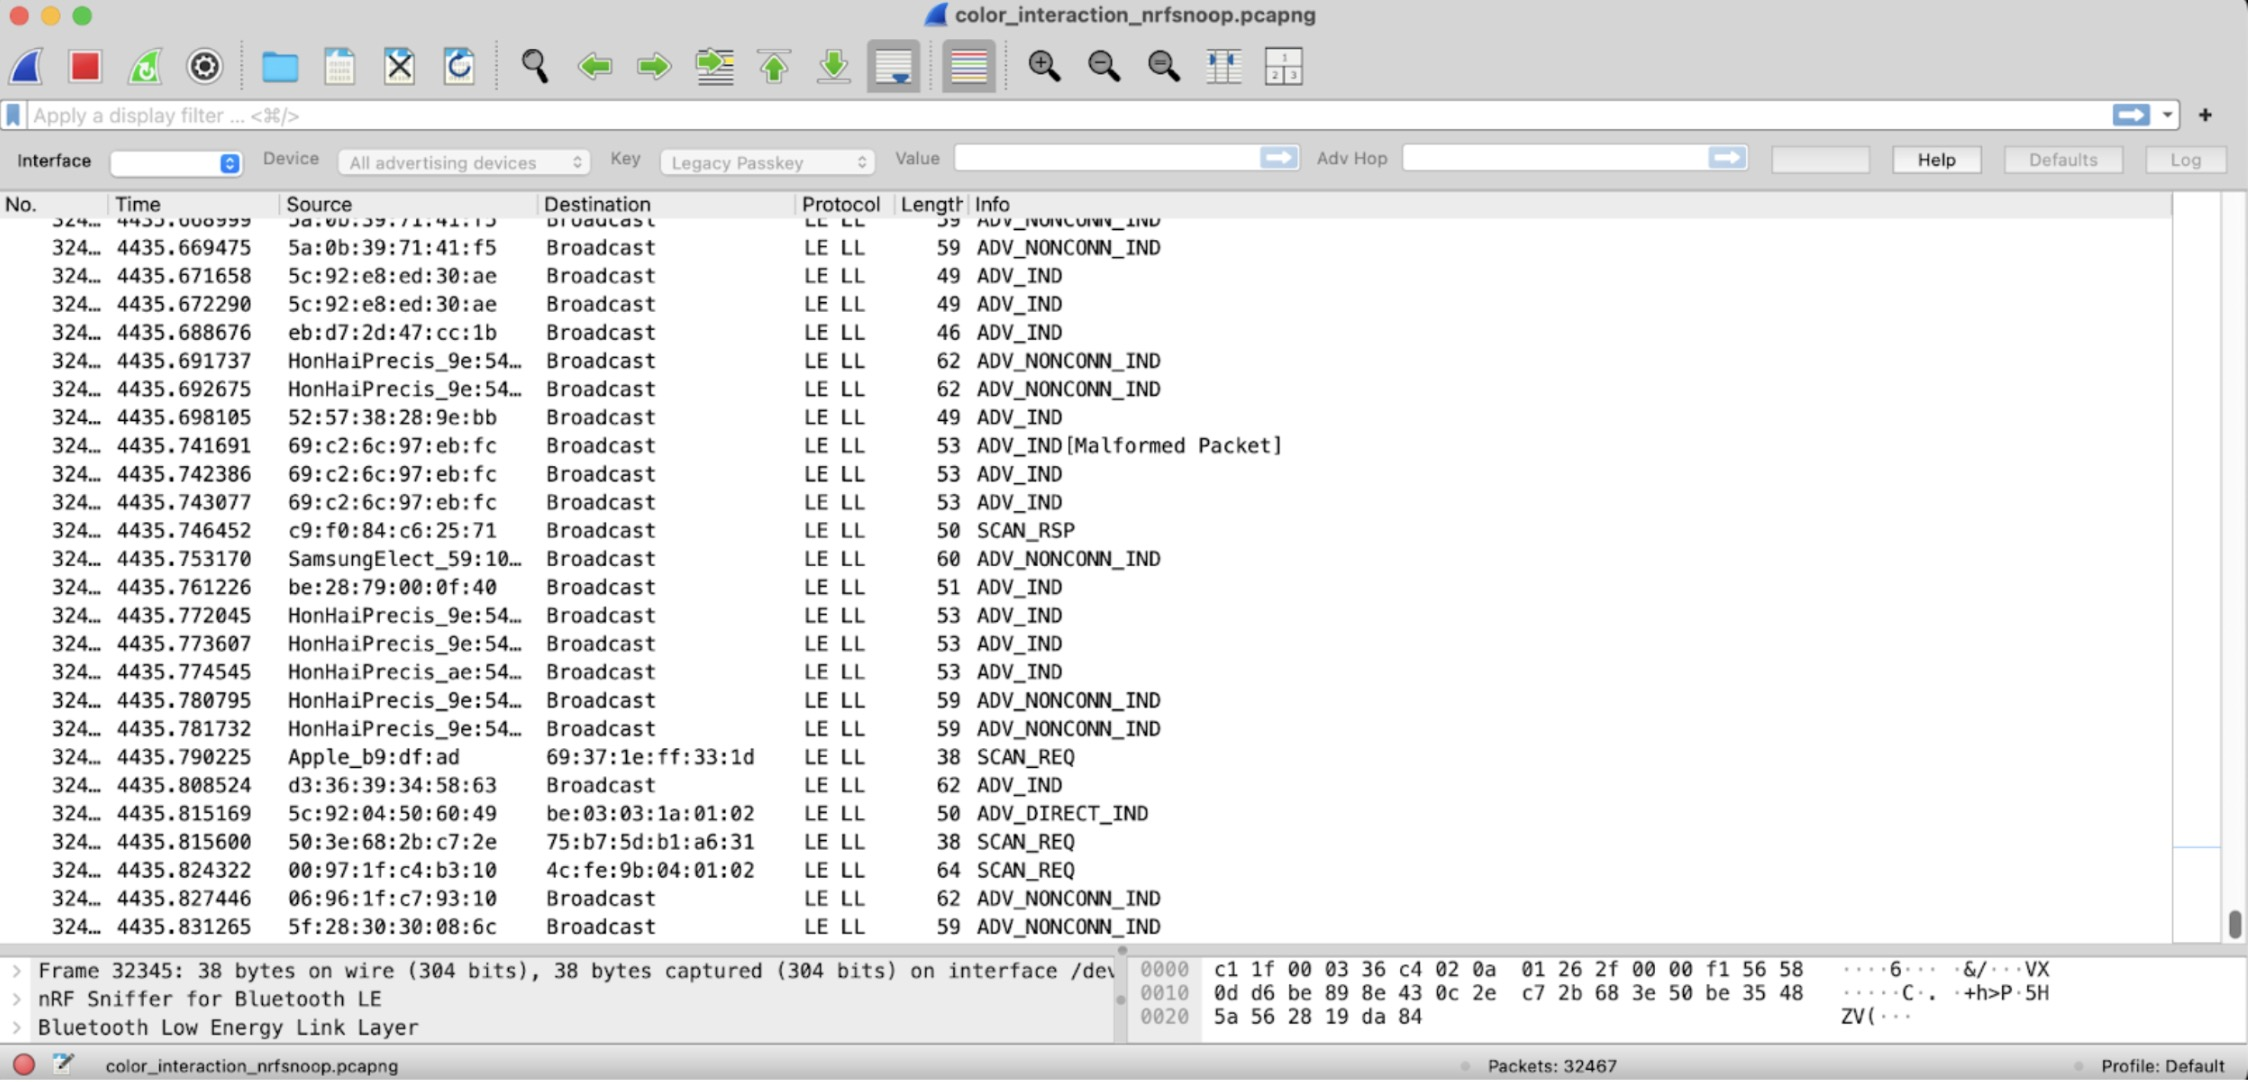
\includegraphics[width=0.7\linewidth]{wireshark_packet_sniffing}
	\caption{Wireshark Output from Bluetooth Packet Sniffing}
	\label{fig:wiresharkpacketsniffing}
\end{figure}

Although Wireshark provides powerful commands for filtering captured data, there was insufficient information to determine suitable filters for isolating the target packets. Attempts to filter based on segments of UUIDs yielded no matches, and manually parsing such a large volume of data was impractical. Fortunately, with an Android device, it is possible to extract HCI snoop logs, which record all of the phone’s Bluetooth interactions. To reduce the volume of data and improve the chances of identifying relevant packets, the next step was to pull these logs directly from the phone.

\section{Analyzing the HCI Snoop Logs}
The first step in obtaining Bluetooth HCI snoop logs is to enable Bluetooth debugging on the device. This requires ensuring that USB debugging is already activated, which should be the case given the extensive ADB debugging performed on the phone thus far. Once confirmed, navigate to the developer settings and enable the option labeled “Enable Bluetooth HCI snoop log.”

With logging enabled, it is then necessary to generate traffic to capture in the log. For my initial test, I chose to record a connection event between the application and the makeup printer device. Retrieving the log from the device proved somewhat more complicated than anticipated, as the file was not stored in the expected location. To locate it, I ran the following command: \textbf{\texttt{find /data -iname '*btsnoop*'}}. This is a prudent step to avoid attempting to pull the log from an incorrect path. Ultimately, the btsnoop log was located in the directory: \textbf{\texttt{/data/misc/bluedroid}}.

Bluedroid is Android’s Bluetooth stack, and files stored in its directories are inaccessible to non-root users due to the system’s permissions model. To retrieve the log, I first copied it to the device’s SD card using the command: \begin{verbatim}
cp /data/misc/bluedroid/2025_05_28_14_24_03_btsnoop.txt /sdcard/btsnoop_hci.log
\end{verbatim}
I then verified the file’s presence on the SD card by executing \textbf{\texttt{ls -l /sdcard/btsnoop\_hci.log}}. Once confirmed, I used the adb pull command to transfer the log to my Mac for further analysis.

With the log successfully copied to the computer, it became ready for examination in Wireshark. To contextualize the data, it is useful to recall the role of Bluetooth’s Host Controller Interface (HCI), which defines the standard communication protocol between the higher-level host and the lower-level controller. Generally, these logs are text files that capture HCI commands, events, and data packets. As a brief reminder, HCI commands are instructions sent from the host to the Bluetooth controller (for example, a disconnect command), while HCI events are the corresponding responses sent from the controller back to the host (for example, a disconnection complete event). Each entry in the log represents a specific communication action or response.
% TODO: \usepackage{graphicx} required
\begin{figure}[H]
	\centering
	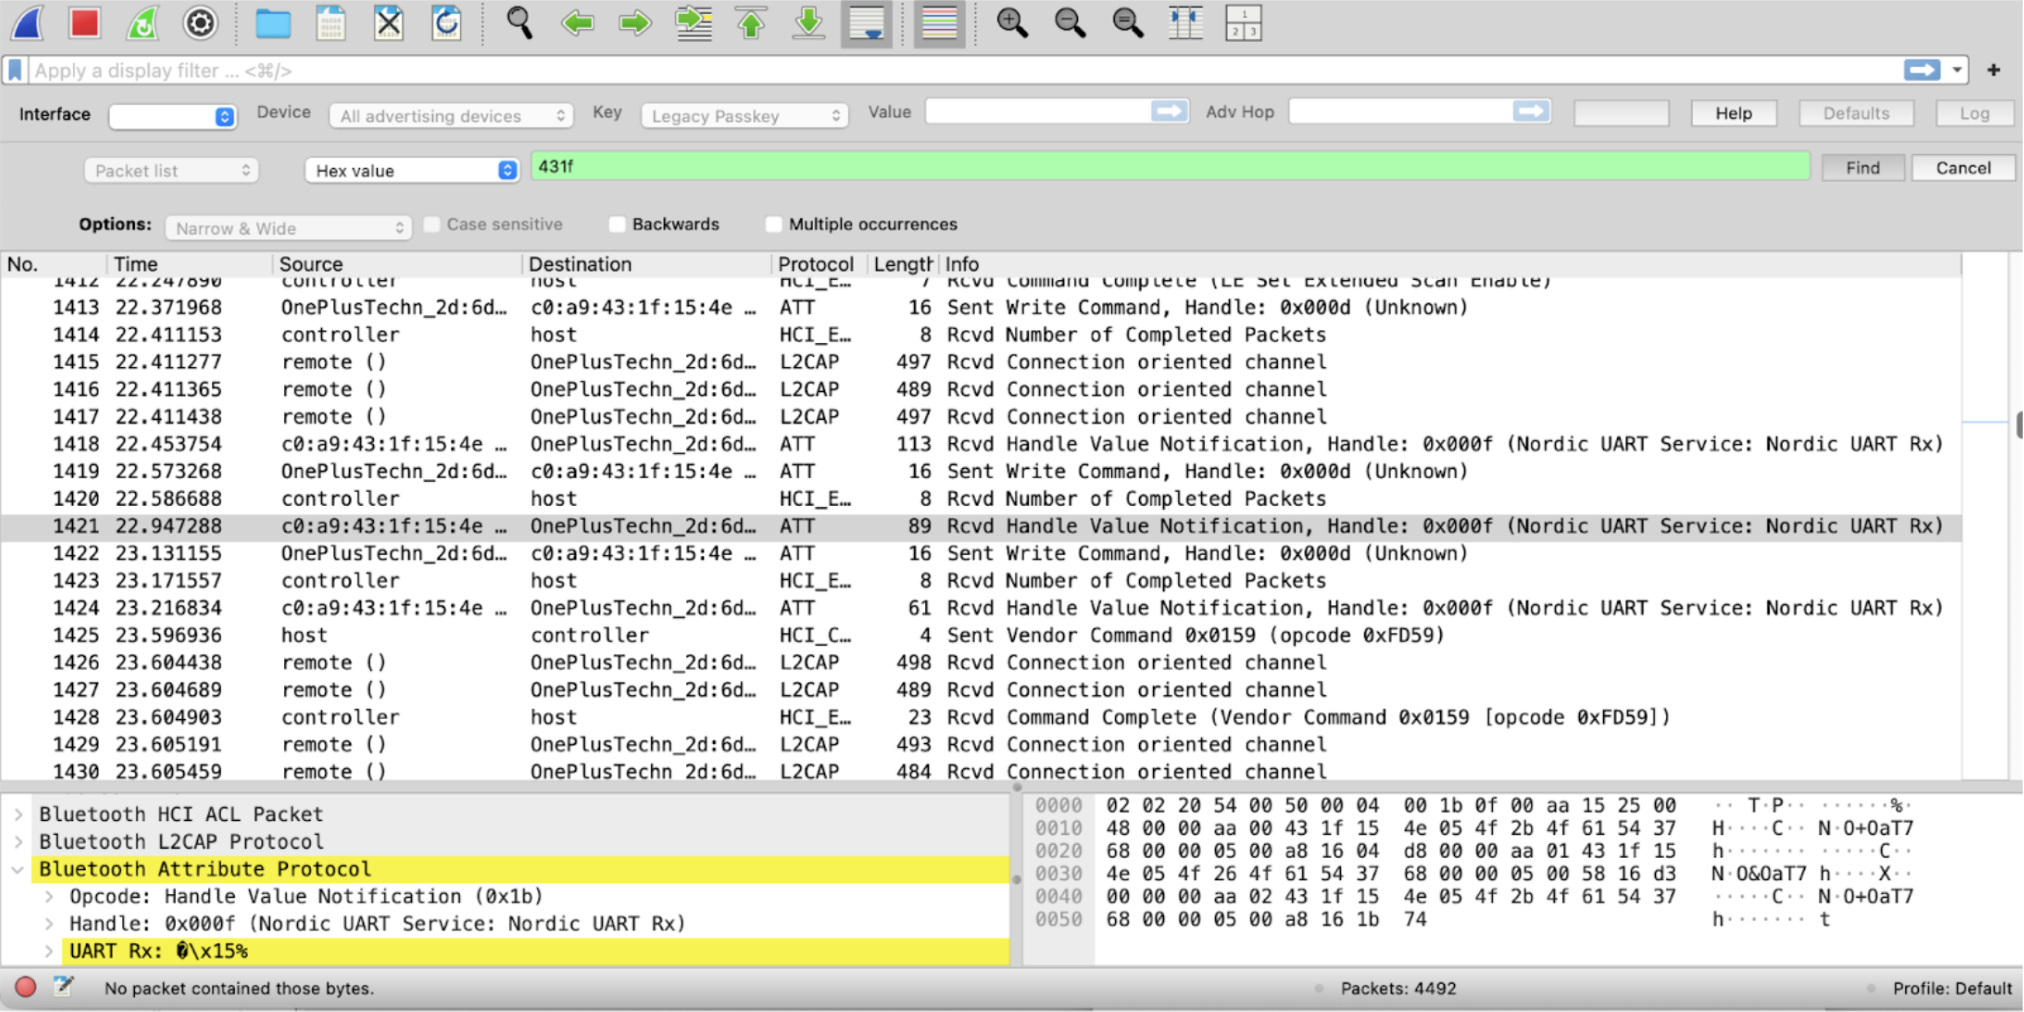
\includegraphics[width=0.7\linewidth]{hci_snoop_log}
	\caption{Wireshark Output from HCI Snoop Logs}
	\label{fig:hcisnooplog}
\end{figure}
Despite filtering the capture to a specific event, the log still contained a substantial number of packets (4,482 in total). To simplify analysis, it is advantageous to use filters within Wireshark. One useful filter for this scenario is the btatt filter, which allows the user to isolate only the Attribute Protocol (ATT) traffic. This protocol governs the discovery, reading, and writing of attributes between a client and a server device.

By narrowing the captured data using this filter, it becomes significantly easier to identify relevant packets that represent interactions between the phone and the device. For instance, in Wireshark I identified communication from the phone, OnePlusTechn\_2d:6d:b6, directed to the device c0:a9:43:1f:15:4e, in which the phone issued a write command.

% TODO: \usepackage{graphicx} required
\begin{figure}
	\centering
	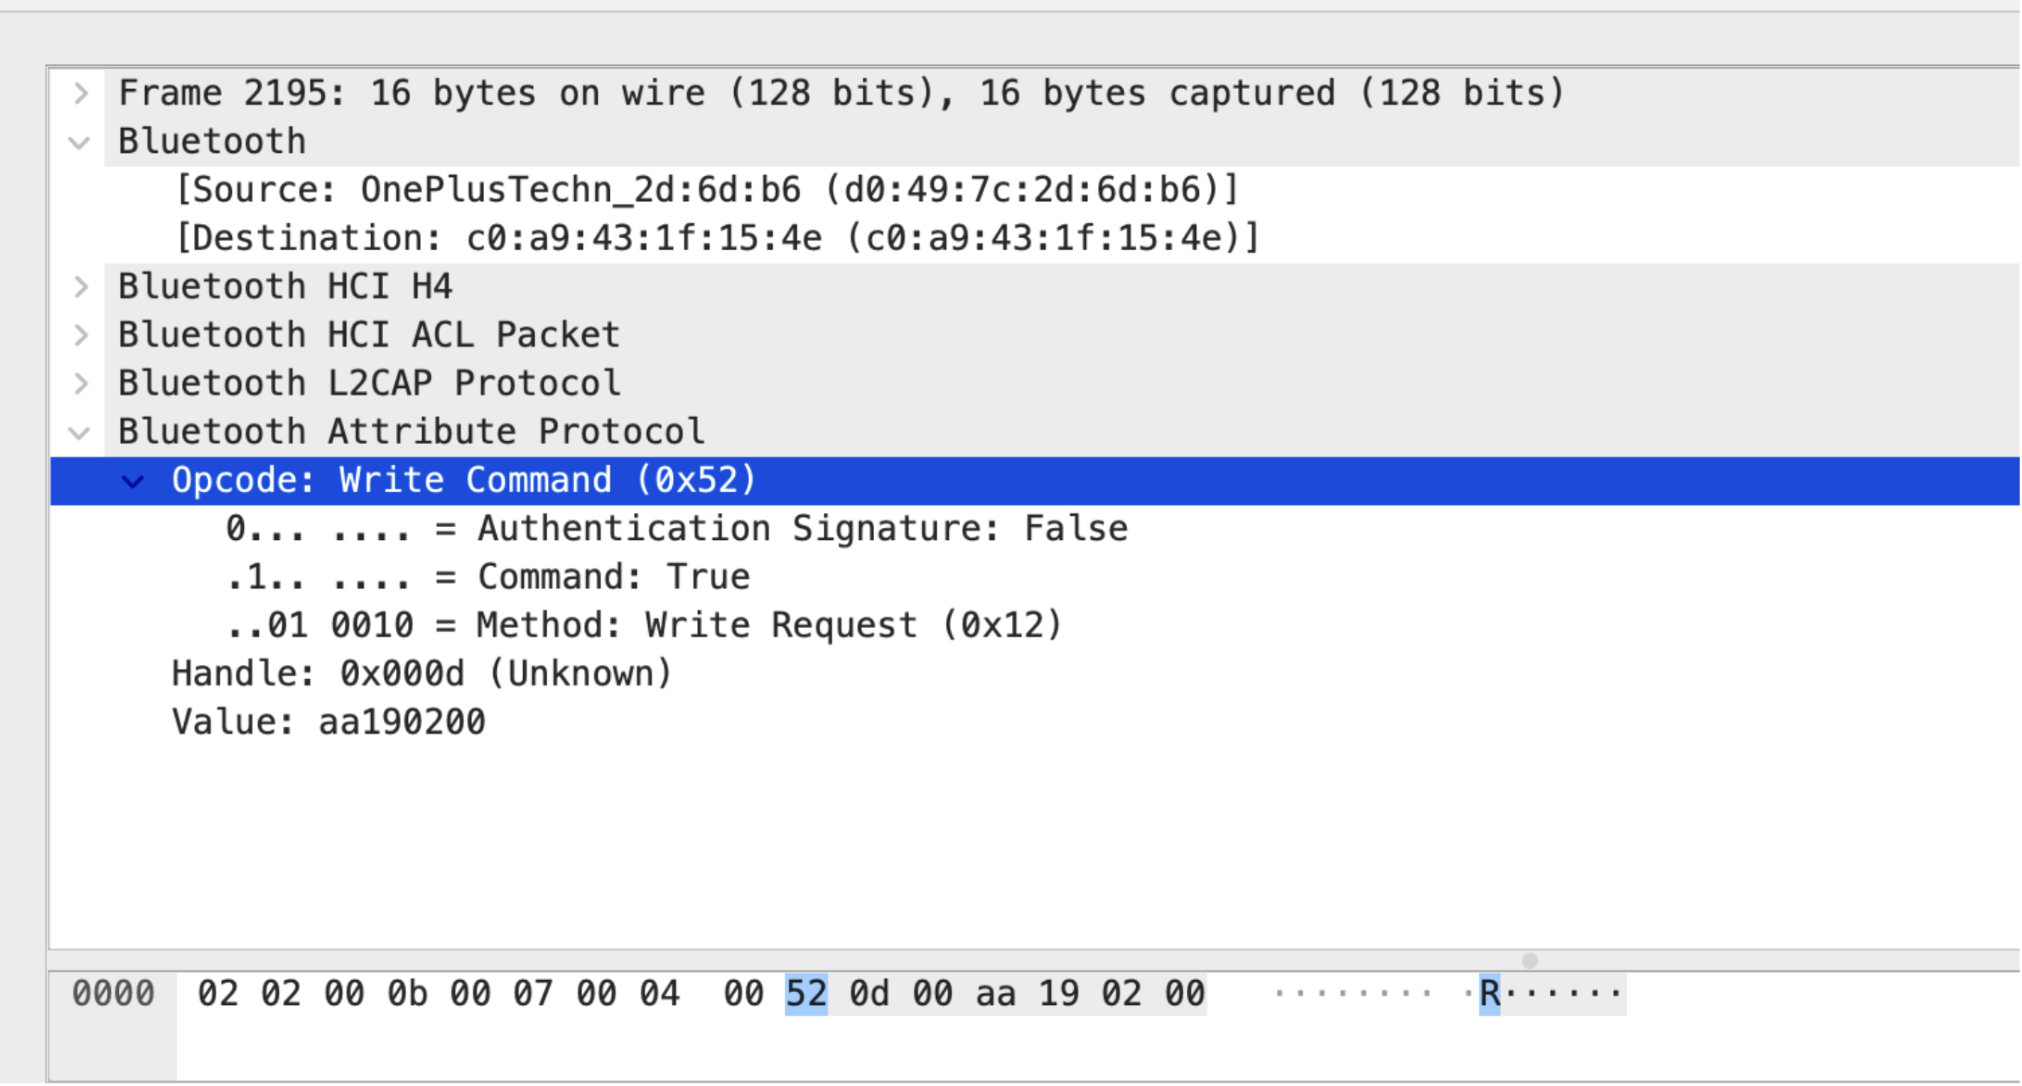
\includegraphics[width=0.7\linewidth]{hci_tree_wireshark}
	\caption{HCI Packet Tree in Wireshark}
	\label{fig:hcitreewireshark}
\end{figure}

By examining the attribute tree in Wireshark, it is possible to locate both the handle and the value of this write operation. In this case, the write occurred to the characteristic with Handle: 0x000d, and the value written was aa190200. To gain a comprehensive understanding of each service and characteristic involved, this analysis process can be repeated for each interaction of interest within the application.

The primary advantage of this method over others is that it reveals low-level Bluetooth interactions occurring on the phone, as well as the bidirectional communication between the device and the phone. Throughout this project, I have found that the ability to dynamically employ various investigative methods as specific challenges arise is critical to the decoding process.

While the information captured in these logs is invaluable, the complexity of the device means that decoding packet data alone would be an excessively time-consuming approach for understanding or modifying the communication. To gain insight into how these packets are constructed and sent, it is necessary to examine the internal functions of the application itself. For this purpose, the next step is to utilize Frida to instrument and analyze the relevant application code.

\section{Scripting}
Frida accomadates the use of scripts to perform specific functions in conjunction with their application. It is a very useful tool in the reverse engineering process to be able to target and extract specific information. The first script created was one to enumerate the contents of the BLE send function. This function is how any and all BLE communications get broadcast through the application so it holds a wealth of information in terms of figuring out how the device is expecting to receive data. While it is hypothetically possible to hook into the Android library's Bluetooth send function, it is much more difficult to do with less payoff than hooking into the native send function. The send() method was discovered by reading through the decompiled code in jadx. Its existence was verified by listing the methods in the BLEManager class using Frida.
\begin{verbatim}
Java.perform(function () {
    var BleManager = Java.use("com.vinsol.loreal.PersoLips.utils.BleManager");
});
\end{verbatim}
Frida has some of its own terminology. \texttt{Java.perform()} is one of the most common Frida methods because it alerts Frida where to hook into the application. Here, Frida is being instructed to hook into the \texttt{BleManager} class.
\begin{verbatim}
    var originalSend = BleManager.send.overload('[B', 'int');
\end{verbatim}
This line saves the original \texttt{send(byte[], int)} function so it can be called as necessary. It will need to be called as usual at the end of enumeration so that there isn’t an interruption in the methods.
	
\begin{verbatim}
function enumerateObject(obj) {
    try {
        var objClass = obj.getClass();
        console.log("Object class: " + objClass.getName());
        
        var fields = objClass.getDeclaredFields();
        for (var i = 0; i < fields.length; i++) {
            var field = fields[i];
            field.setAccessible(true);
            try {
                var name = field.getName();
                var value = field.get(obj);
                console.log("  Name: " + name + " = " + value);
            } catch (err) {
                console.log(" Could not access field: " + err);
            }
        }
    } catch (err) {
        console.log("Error during enumeration: " + err);
    }
}
\end{verbatim}
This is the definition for the function to enumerate the contents of each object in the \texttt{send()} function. The \texttt{try\{\}}/\texttt{catch\{\}} allows the function to execute safely without crashing. The \texttt{getClass} Java method gets the class of the object at runtime. It then loops through each field and sets them as accessible. For each field in the loop, it logs the name and object value.
\begin{verbatim}
BleManager.send.overload('[B', 'int').implementation = function (bArr, i) {console.log("send() called with device ID: " + i);
\end{verbatim}
Here is where the \texttt{send} function actually gets overridden. It starts by logging that the \texttt{send} function was called.
\begin{verbatim}
var bytes = Java.array('byte', bArr);
var hex = Array.from(bytes).map(function (b) {
return ('0' + (b & 0xFF).toString(16)).slice(-2);
}).join(' ');
console.log("Payload (hex): " + hex);
\end{verbatim}
This code segment is where the byte array output of \texttt{send} gets converted into hex to make it easier to read. It starts by turning the Java byte array \texttt{bArr} into a format that can be read by Frida. The bytes are then ANDed with \texttt{0xFF} to convert signed bytes to unsigned. It then converts the result into base 16 (hex). Finally, \texttt{slice(-2)} ensures each value is represented by two characters (zero-padded if needed).
\begin{verbatim}
console.log("Enumerating fields of BleManager instance...");
enumerateObject(this);
\end{verbatim}
This logs and inspects the current \texttt{BleManager} instance — the object calling \texttt{send()}. It gives insight into the app’s internal state at the moment of the call.
\begin{verbatim}
return originalSend.call(this, bArr, i);
\end{verbatim}
Finally, the original \texttt{send()} function is called to allow normal app behavior to continue uninterrupted.

\section{Analyzing BLE Payloads via Frida Hooking and Packet Inspection}
When using Frida for packet analysis, the first and most crucial step is ensuring that I can capture the packet data along with any functions I intend to hook. Fortunately, this is achievable directly within Frida by identifying where Android’s writeCharacteristic function is implemented. This function is responsible for transmitting data over Bluetooth Low Energy (BLE). By using JADX, I was able to locate this function without much difficulty in the BleManager class, as discussed in the scripting section. Within this class, the relevant method is appropriately named \texttt{send()}.

With the app’s \texttt{send()} method hooked, I was able to perform various tests where I made small alterations to the dispense output to observe how these changes affected the raw payload. I experimented with modifications to color, volume, and dispense time, hoping to identify clear RGB values within the packet alongside the corresponding volume information for each print command. Based on research into other color-based BLE devices, such as LED lights, these values often appear clearly in some portion of the payload.
Unfortunately, this device proved to be more complex. Given the novelty of the technology and the significant investment behind its production, this complexity is not surprising. While the Bluetooth communications were not encrypted, they were intricate enough that simply knowing what the device was supposed to do was not sufficient; a deeper understanding of the app’s source code was necessary.

One drawback of hooking the \texttt{send()} function instead of using a finely tuned Bluetooth sniffer was that I was only able to capture the communications that the hook managed to log. This excluded packets received from the device. Additionally, the timing of these logged transmissions might not be entirely accurate since they are not captured immediately but rather passed through the hook. Although I had access to a Bluetooth packet sniffer, the output was overly verbose, filled with external Bluetooth noise, and ultimately too time-consuming to filter within the constraints of my project. Time constraints often lead to the abandonment of reverse engineering efforts, so given the number of time-intensive tasks involved, I opted to prioritize monitoring the send() function even at the cost of some fidelity.

To get a more complete view of the Bluetooth communication, I later hooked the app’s onCharacteristicChanged() function, which logs changes to a Bluetooth Service's Characteristic. This allowed me to track device-side byte payloads and gain a better understanding of the full communication process between the phone (central) and the device (peripheral).

The first step in decoding the payload was to investigate what was happening between the sends. Frida provides a helpful function for this called getStackTraceString(). However, Frida’s documentation can be sparse and often difficult to navigate without prior experience. Fortunately, others have encountered similar issues and created cheat sheets and niche guides for many common Android reverse engineering tasks. Figure \ref{fig:hookedpayload} is an example from an early test. The call stack was generated by triggering an exception, which Frida then intercepted to return the stack values:
% TODO: \usepackage{graphicx} required
\begin{figure}[H]
	\centering
	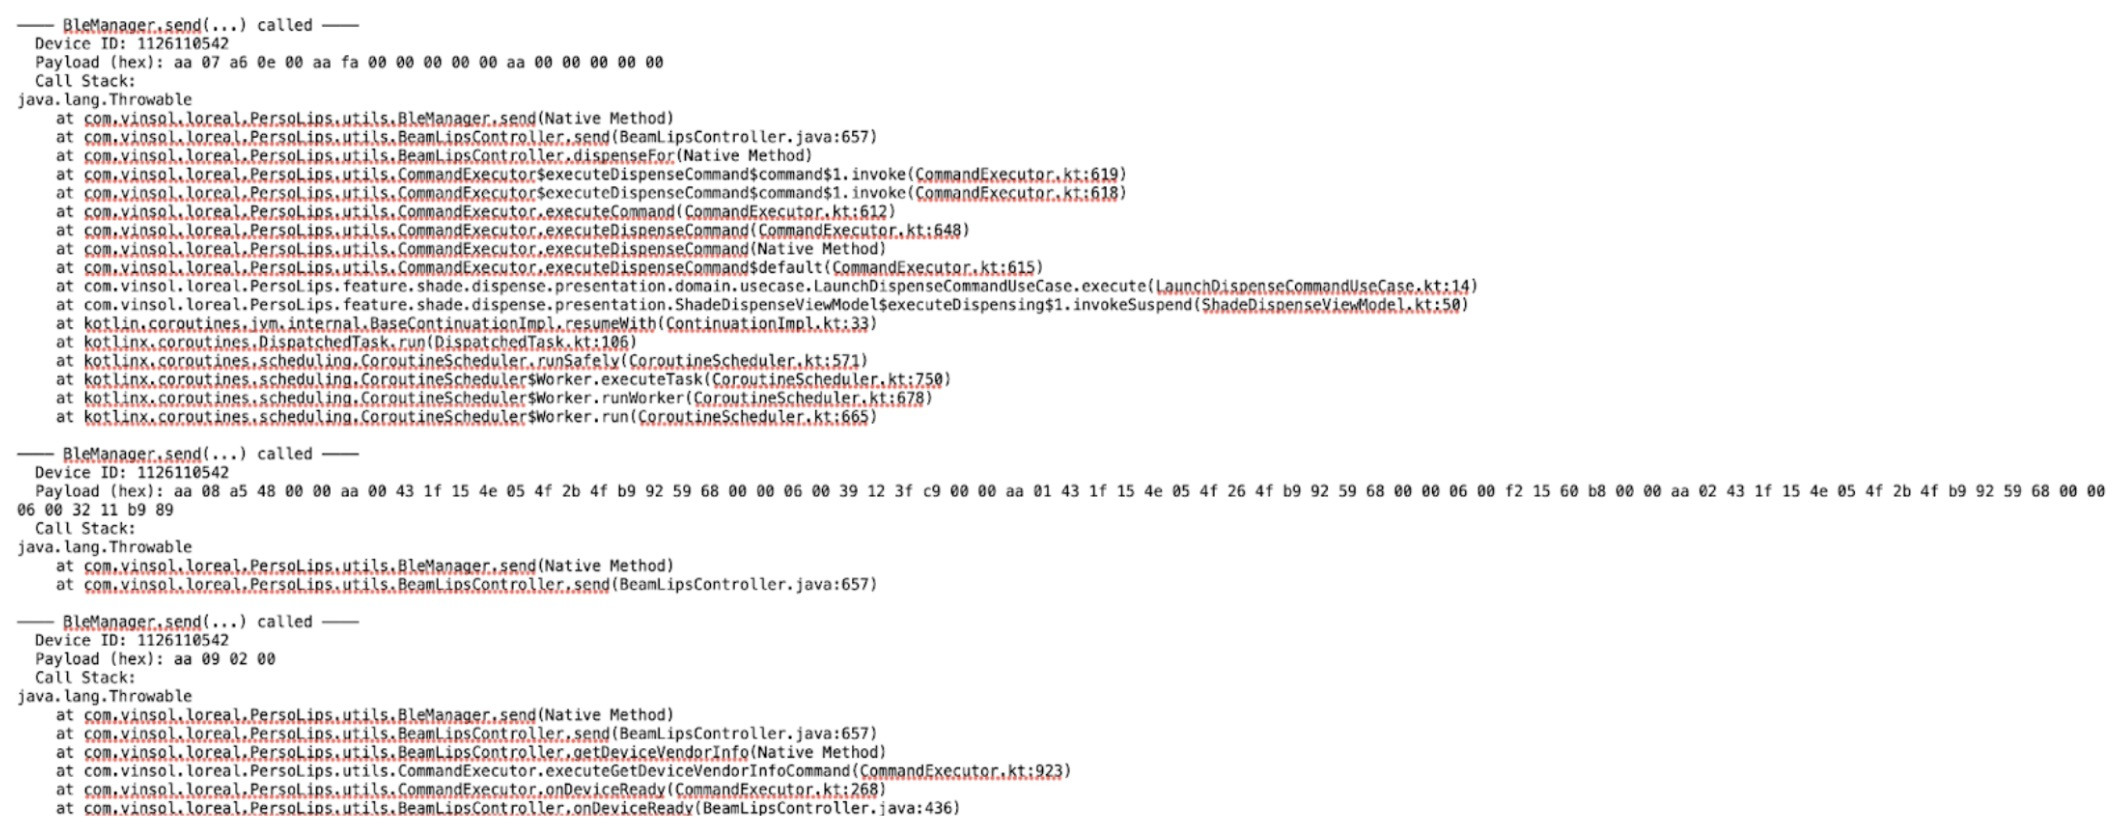
\includegraphics[scale=.225]{hooked_payload}
	\caption{Payload from Hooked Send Method}
	\label{fig:hookedpayload}
\end{figure}

This stack trace offered strong clues about which packages to examine for more dispensing information. However, there was still a significant amount of investigation required. For example, the first method visible aside from \texttt{send()} was \texttt{dispenseFor()}. This is a native method, which means it is implemented in a language other than Java and compiled for a specific computer architecture, usually in C or C++. Native methods can access system-specific APIs not directly available in Java. According to IBM, “Native methods are Java™ methods that start in a language other than Java. Native methods can access system-specific functions and APIs that are not available directly in Java” \cite{ibmNativeMethods}. These methods are stored in \texttt{.so} files within the APK and cannot be decompiled with Dalvik bytecode decompilers like JADX. Instead, they must be reverse engineered from assembly-level code, which is possible but time-consuming. Because of this, I chose to focus on gathering more context through dynamic analysis rather than attempting to decompile the native code.  

To begin understanding the \texttt{dispenseFor()} function, I examined its declaration in JADX and logged its parameters. The only reference to it outside the \texttt{executeDispense()} function appeared in the BeamLipsController: \textbf{\texttt{public native int dispenseFor(int i, String str, int i2, int i3, int i4, float f, int i5);}}
This signature provided insight into the types of variables used. The reference within executeDispense() offered a clearer picture of the parameters: \texttt{beamLipsController.dispenseFor(beamLipsDeviceId, colorUniverse, Color.red(color), Color.green(color), Color.blue(color), floatValue, intValue);}
This helped identify the values that would need to be verified during testing. Below is the Frida hook I implemented to intercept calls to dispenseFor() and log the relevant information:
\begin{verbatim}
	// Hook dispenseFor(...)
	BeamLipsController.dispenseFor.overload(
	'int', 'java.lang.String', 'int', 'int', 'int', 'float', 'int'
	).implementation = function (deviceId, colorUniverse, r, g, b, vol, dose) {
		console.log("\n--- dispenseFor(...) called ---");
		console.log("  Device ID: " + deviceId.toString(16));
		console.log("  Color Universe: " + colorUniverse);
		console.log("  Red: " + r + " | Green: " + g + " | Blue: " + b);
		console.log("  Volume (float): " + vol + " → " + toHex(floatToBytes(vol)));
		console.log("  Dose (int): " + dose + " → " + toHex(intToBytes(dose)));
		console.log("  Call Stack (starting with exception):\n" +
		Log.getStackTraceString(Exception.$new()));
		logObjectFields(this);
		
		return this.dispenseFor(deviceId, colorUniverse, r, g, b, vol, dose);
	};
\end{verbatim}
And below is the resulting output from the test (excluding the call stack for brevity). 
\begin{verbatim}
	--- dispenseFor(...) called ---
	Device ID: 431f154e
	Color Universe: cool_nude
	Red: 228 | Green: 101 | Blue: 135
	Volume (float): 0.07999999821186066 -> 3d a3 d7 0a
	Dose (int): 1 -> 00 00 00 01
\end{verbatim}
\begin{table}[H]
\centering
\caption{Cartridge Metadata and Status at Time of Dispense}
\label{tab:cartridgedata}
\begin{scriptsize}
\begin{tabular}{|l|l|l|l|}
\hline
\textbf{Field} & \textbf{Cartridge 0} & \textbf{Cartridge 1} & \textbf{Cartridge 2} \\
\hline
Type & 00 & 00 & 00 \\
PCrc16 & DBB13410 & 8E0746A3 & 258719E9 \\
Volume & 4.165000 & 5.618000 & 4.084000 \\
Crc16 & DD21 & CF18 & B1CC \\
DeviceId & 431F154E & 431F154E & 431F154E \\
TubeId & 0 & 1 & 2 \\
Last use & 2025-06-26 01:29:16 & 2025-06-26 01:29:16 & 2025-06-26 01:29:16 \\
Open date & 2025-05-20 08:00:00 & 2025-05-20 08:00:00 & 2025-05-20 08:00:00 \\
End date & 2025-06-27 08:00:00 & 2025-06-22 08:00:00 & 2025-06-27 08:00:00 \\
Exp. date & 2025-06-27 08:00:00 & 2025-06-22 08:00:00 & 2025-06-27 08:00:00 \\
Formula id & MA\_513 & MA\_200 & MA\_100 \\
Usable Vol. & 5.800000 & 5.800000 & 5.800000 \\
Duration use & 730 & 730 & 730 \\
Prod date & 2022-06-28 08:00:00 & 2022-06-23 08:00:00 & 2022-06-28 08:00:00 \\
Batch id & 62W601 & 62W601 & 62W601 \\
Color & 00DF75A0 & 006A2623 & 00C8725C \\
Present? & 1 & 1 & 1 \\
Up to date? & 1 & 1 & 1 \\
Compatible? & 1 & 1 & 1 \\
Opened? & 1 & 1 & 1 \\
Expired? & 0 & 1 & 0 \\
Empty? & 0 & 0 & 0 \\
Valid? & 1 & 1 & 1 \\
Virtual? & 0 & 0 & 0 \\
CanDispense? & 1 & 1 & 1 \\
\hline
\end{tabular}
\end{scriptsize}
\end{table}
It is clear that much of the information required for the dispensing process is stored within the BeamLipsController object. While examining the JADX decompilation, I found that many of these fields also appear in the BeamLipsDevice model:

% TODO: \usepackage{graphicx} required
\begin{figure}[H]
	\centering
	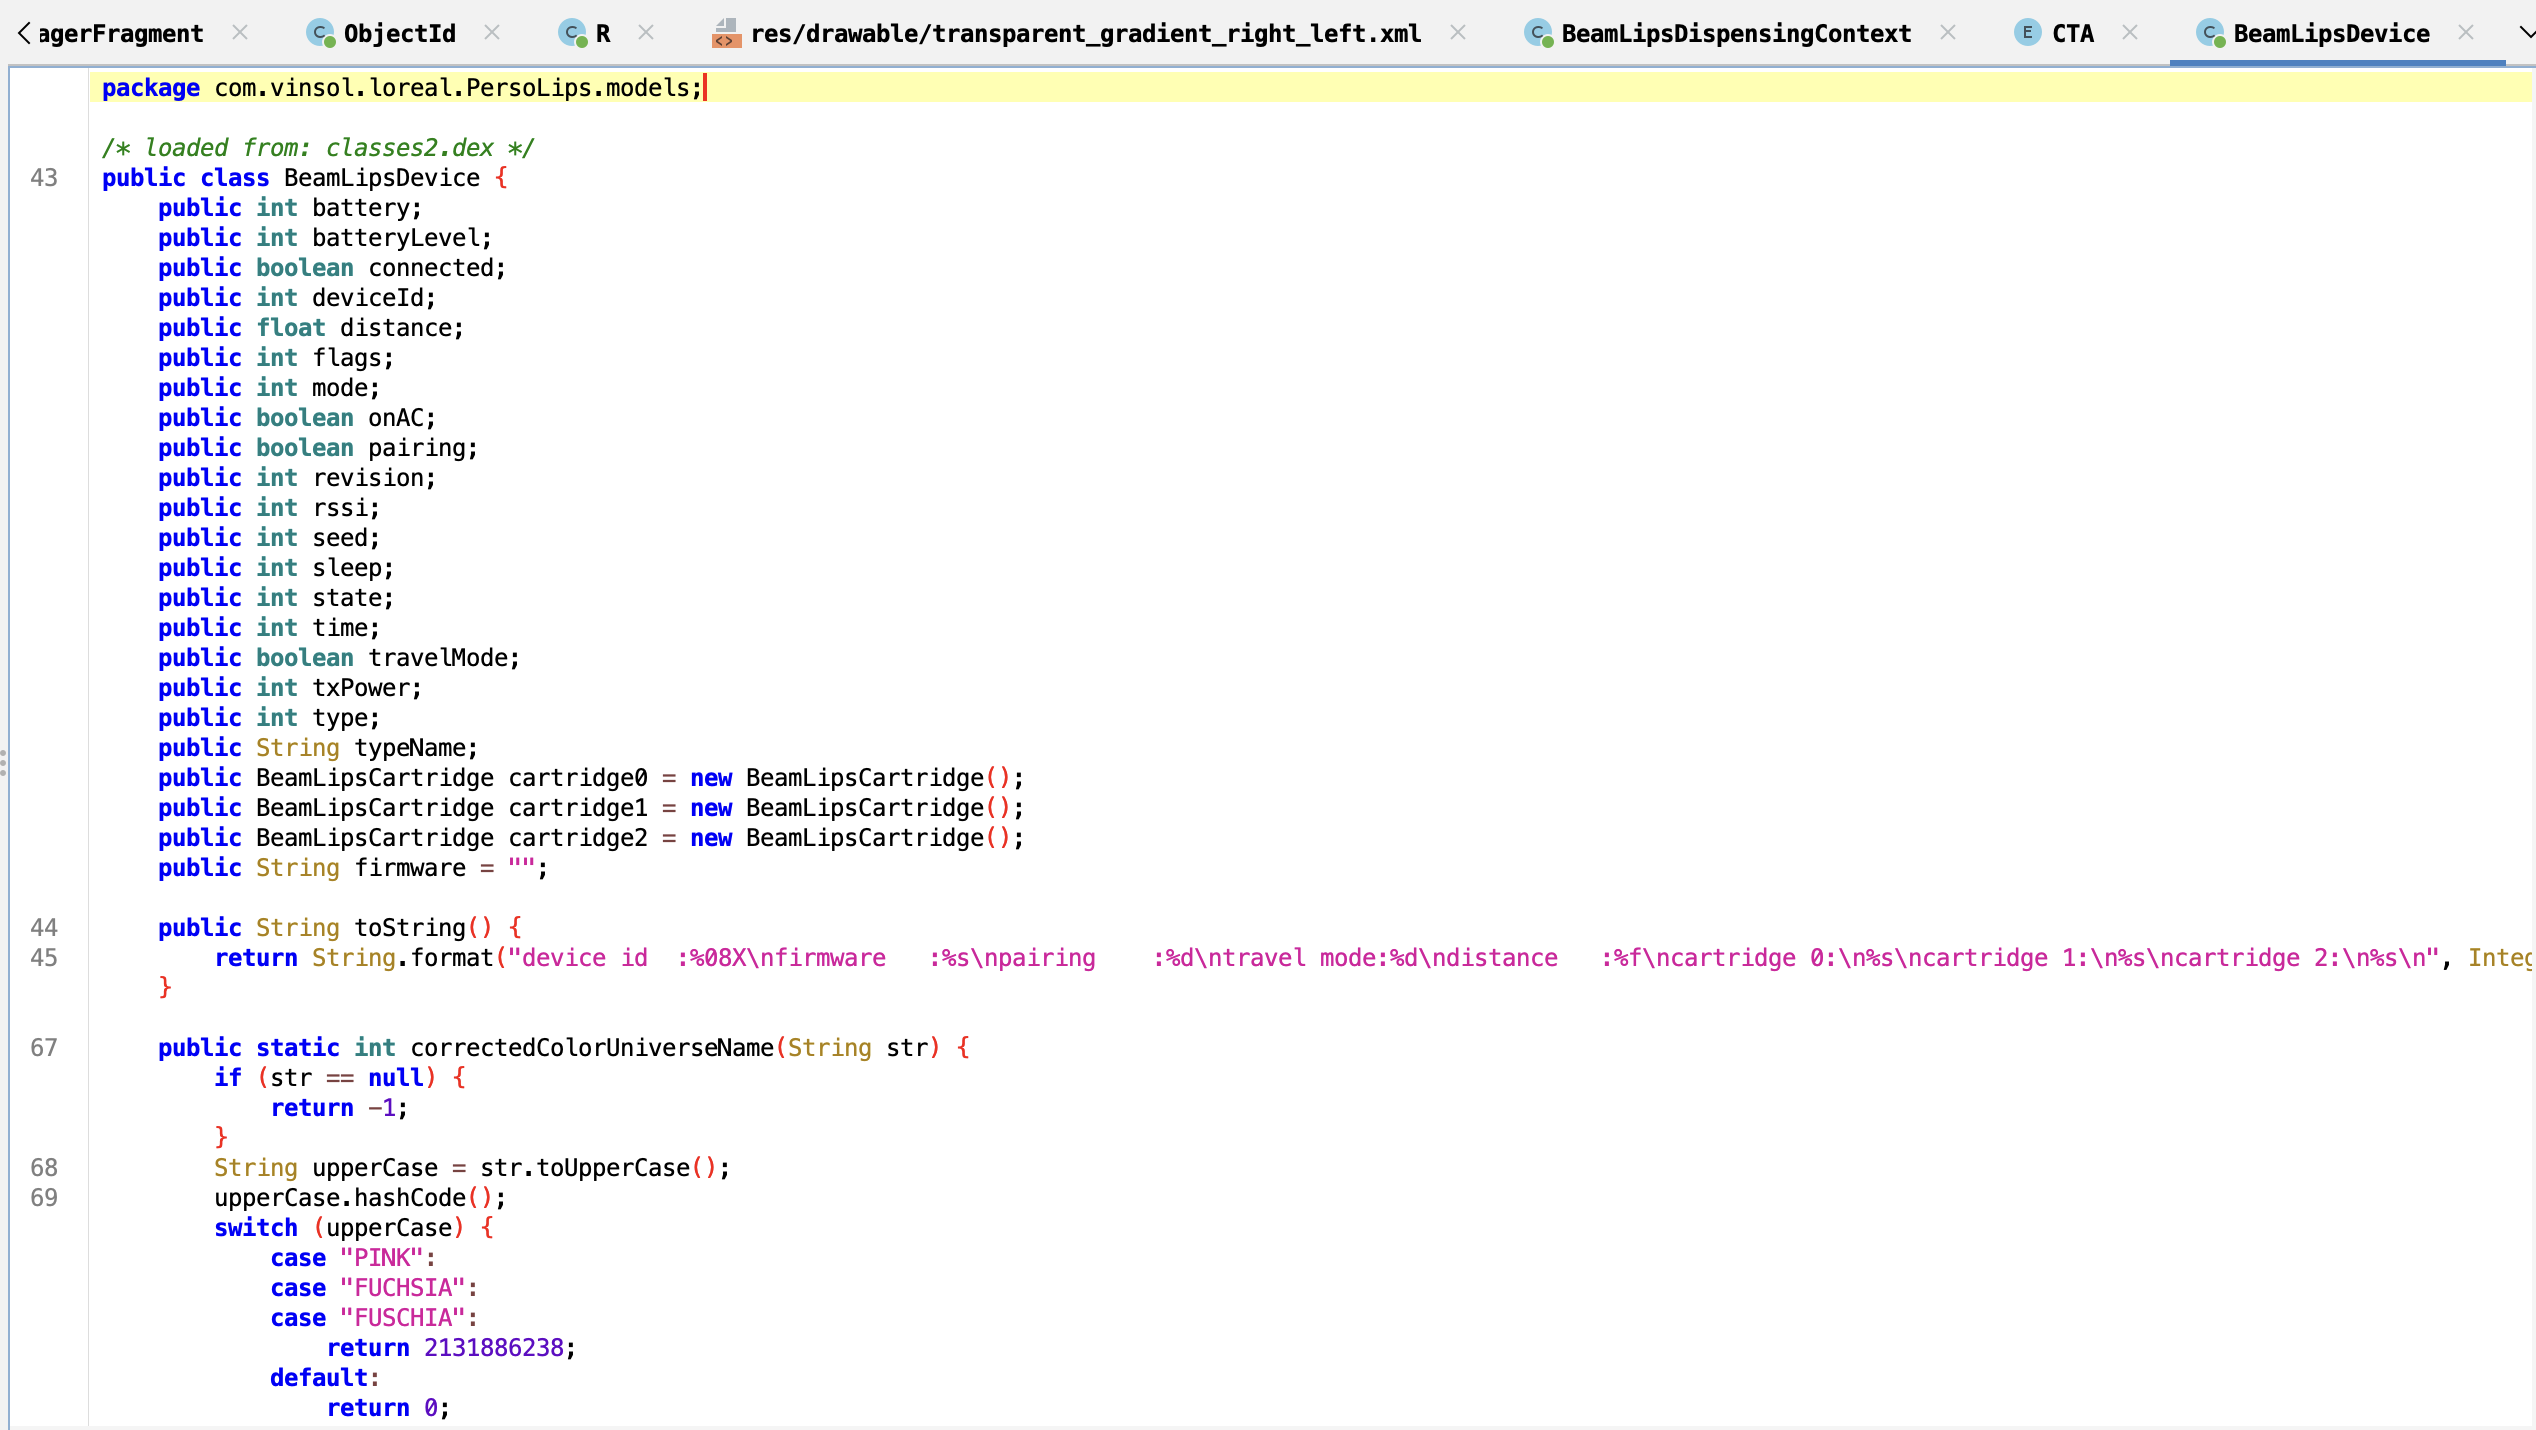
\includegraphics[width=0.7\linewidth]{beamlipsmodel}
	\caption{Beam Lips Device Model Jadx}
	\label{fig:beamlipsmodel}
\end{figure}

These variables provide valuable clues about what to look for in the raw payload. A crucial detail is that the device information appears to be divided into three cartridges, each maintaining its own set of data. Among the variables that seem particularly relevant to the dispense function are the usable volume, color, and dispense duration. I made note of these values to check whether they could be identified within the payload.

With these values hooked, the next step was to run tests and analyze the outcomes. After altering the variables, I was able to trace how specific values appeared in the payload. For example, the dispense payload associated with the dispenseFor hook revealed several important patterns:

% TODO: \usepackage{graphicx} required
\begin{figure}[H]
	\centering
	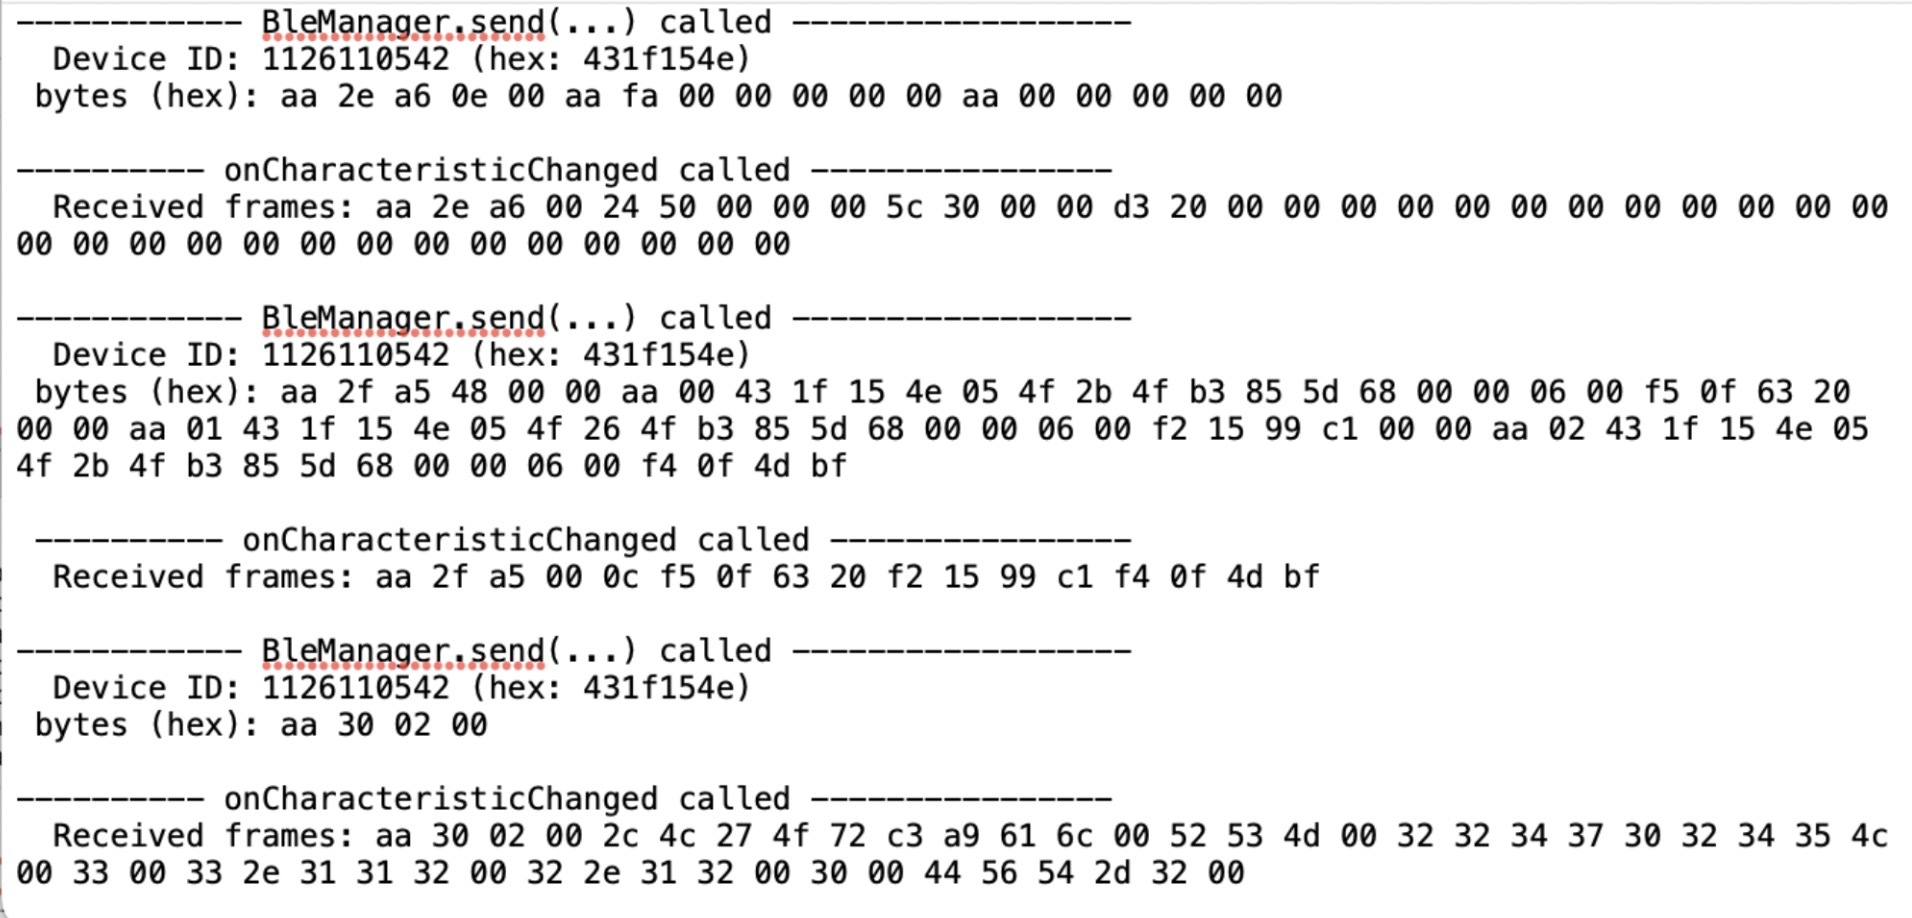
\includegraphics[width=0.7\linewidth]{payload1}
	\caption{Initial Payload from dispenseFor(...) Hook}
	\label{fig:payload1}
\end{figure}

One of the first observations was that each \texttt{send()} transmission began with the byte aa, followed by a byte that incremented with each new message (e.g., 2e, 2f, 30). This indicates that the first two bytes of each payload likely serve as a counter to keep track of the sequence of transmitted packets. Additionally, after the app sends these two bytes (such as aa 2e), the device responds by writing back the same two bytes, further supporting the idea that this sequence acts as a counter and confirmation mechanism to ensure messages are being received in the correct order.

Another significant detail was that the device ID appeared three times in the second \texttt{send()} payload. Figure \ref{fig:deviceid} shows a screenshot of the device’s advanced settings screen from the app, which aligns with earlier findings from the hook indicating that the device splits its data into three channels, one for each cartridge. However, I continued investigating to determine whether any additional relevant information was present in the larger send() packet:

% TODO: \usepackage{graphicx} required
\begin{figure}[H]
	\centering
	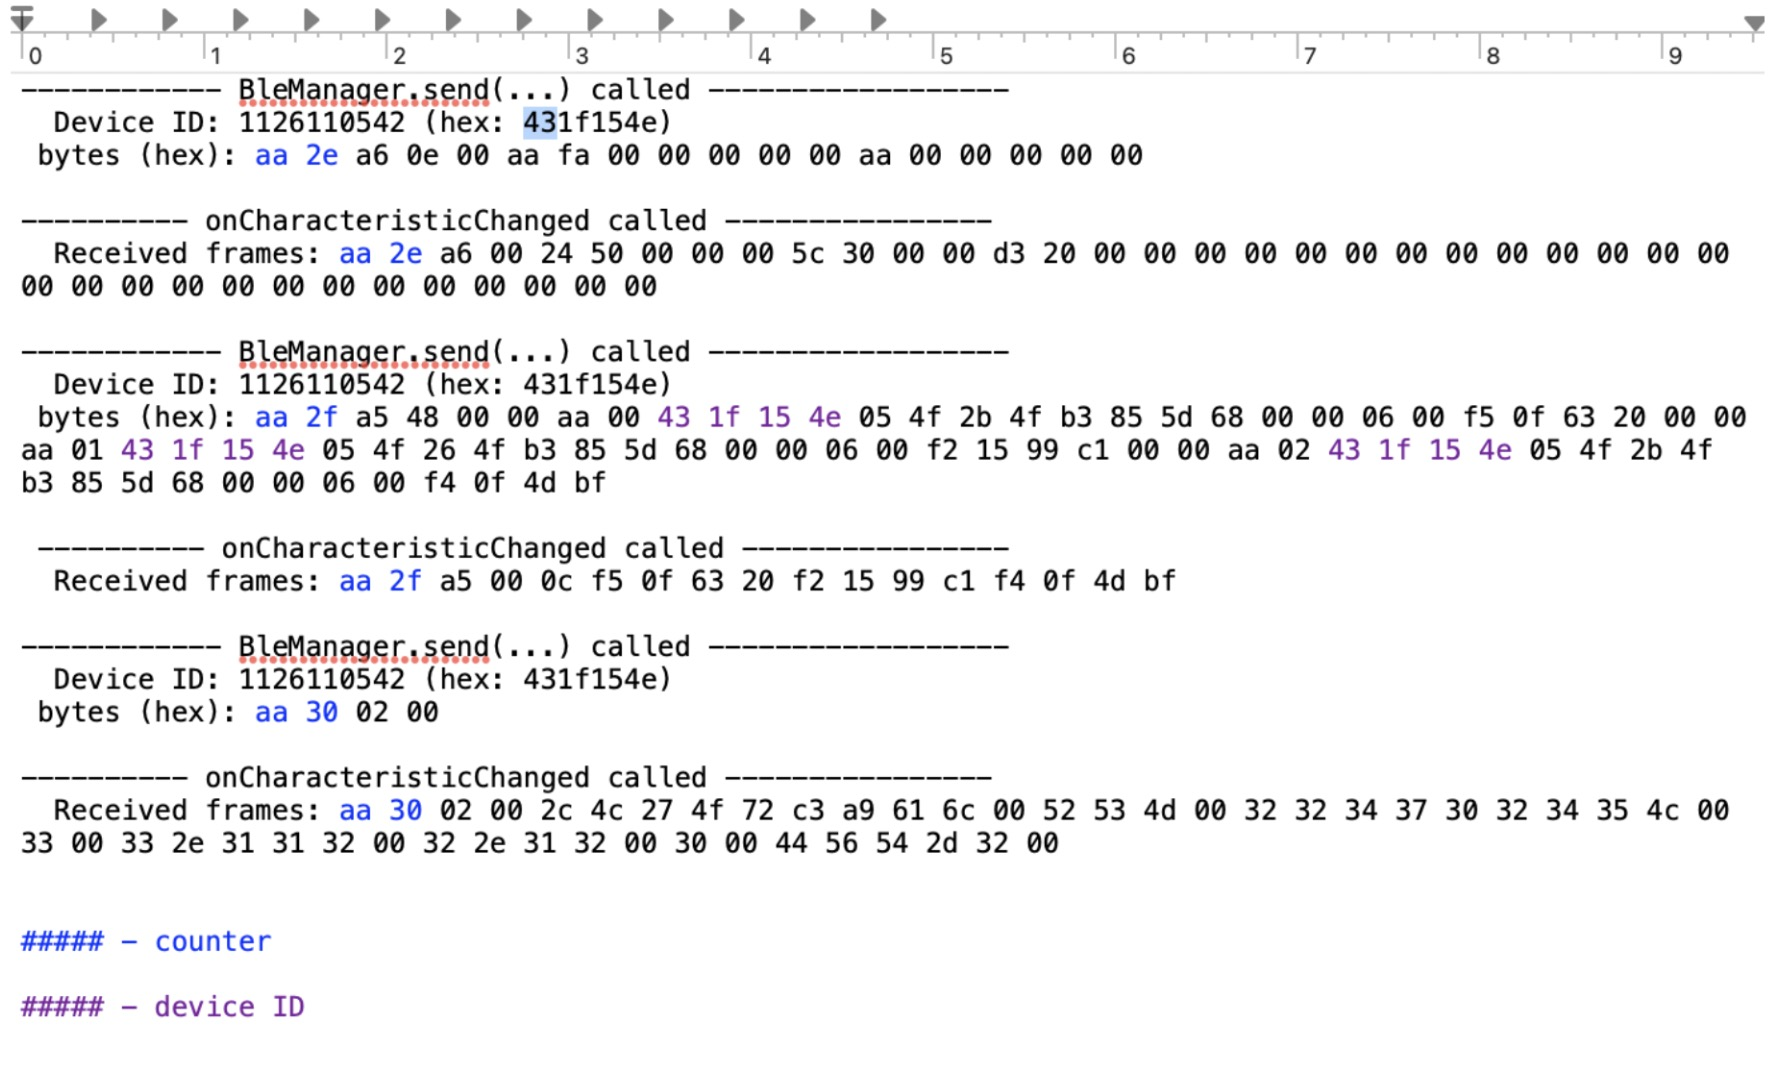
\includegraphics[width=0.7\linewidth]{payload2}
	\caption{Payload Two from dispenseFor(...) Hook}
	\label{fig:payload2}
\end{figure}

% TODO: \usepackage{graphicx} required
\begin{figure}[H]
	\centering
	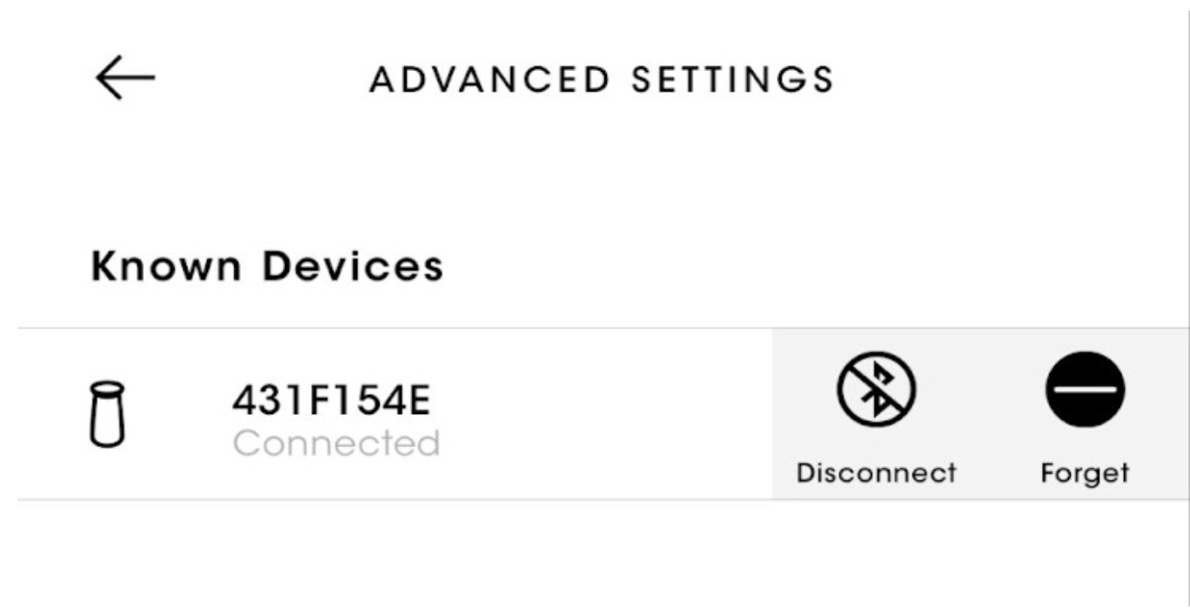
\includegraphics[width=0.7\linewidth]{device_id}
	\caption{Device ID from the App}
	\label{fig:deviceid}
\end{figure}

Working from the hypothesis that the large send payload is organized by cartridge, I continued parsing through the data. As anticipated, I identified the patterns aa 00, aa 01, and aa 02 preceding each occurrence of the device ID, suggesting that the subsequent bytes are associated with data for each cartridge.

It is important to note that, while the information is presented here in a relatively straightforward manner, confirming each hypothesis required numerous tests and careful analysis:

% TODO: \usepackage{graphicx} required
\begin{figure}[H]
	\centering
	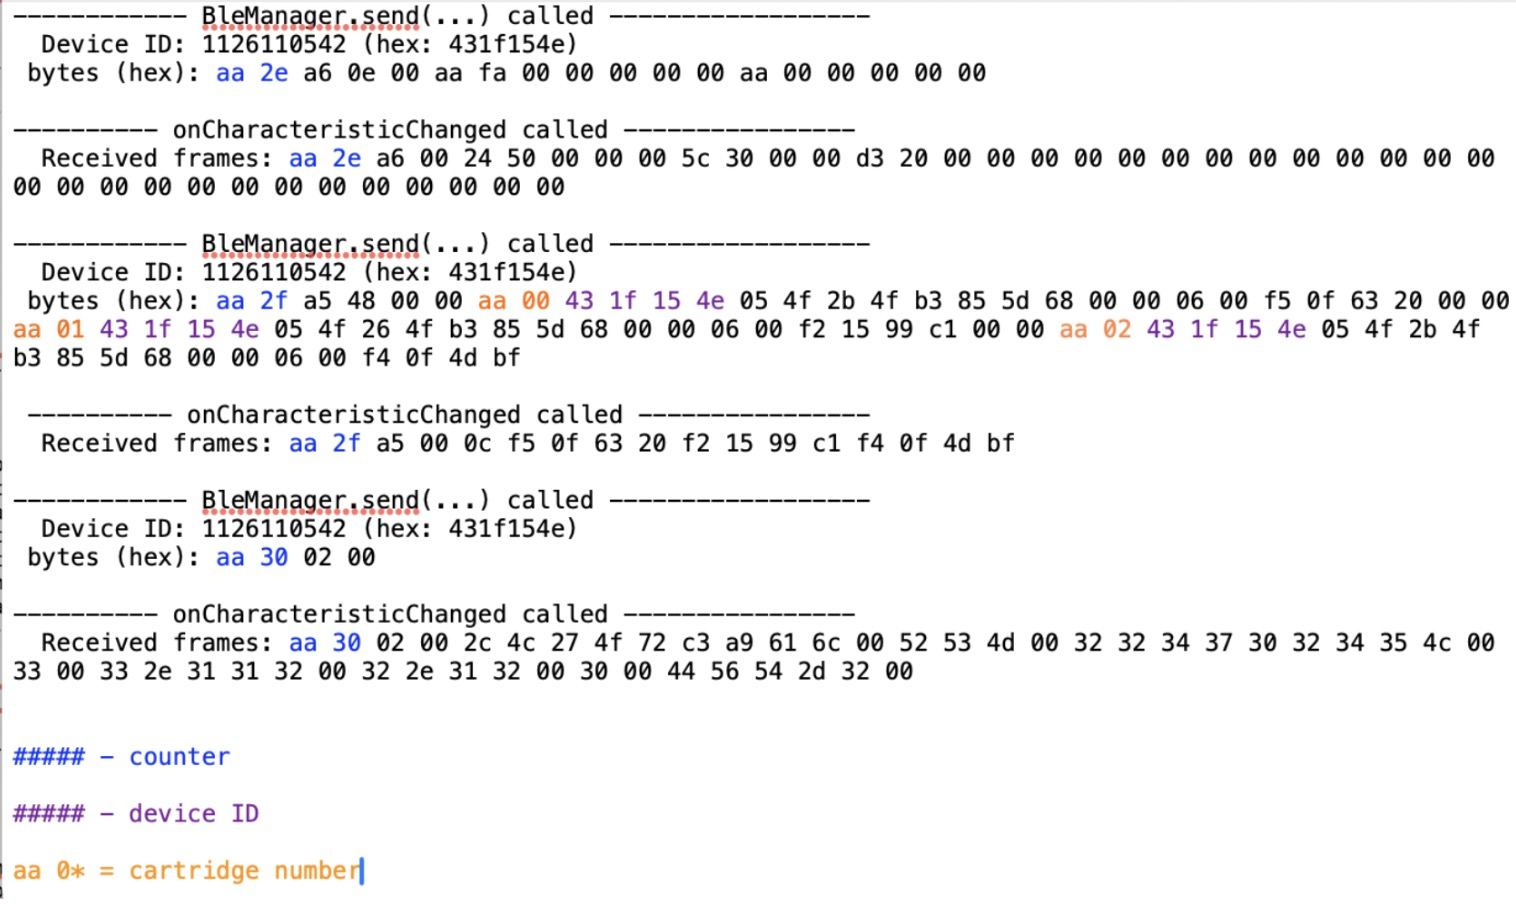
\includegraphics[width=0.7\linewidth]{payload3}
	\caption{Payload Three from dispenseFor(...) Hook}
	\label{fig:payload3}
\end{figure}

This is where the analysis began to grow more complex. To start, it’s important to understand the expected order in which the data appears. As a reminder, the send() and receive payloads under examination here are part of Bluetooth’s GATT profiles. According to the Bluetooth Core Specification 6, the GATT framework “defines procedures and formats of services and their characteristics. The procedures defined include discovering, reading, writing, notifying and indicating characteristics, as well as configuring the broadcast of characteristics” ~\cite{bluetooth2023}. The specification also states that “Multi-octet fields within the GATT profile shall be sent least significant octet first (little-endian) with the exception of the Characteristic Value field. The Characteristic Value and any fields within it shall be little-endian unless otherwise defined in the specification which defines the characteristic” ~\cite{bluetooth2023}. This indicates that much of the data should be expected in little-endian format.

Revisiting the payload, the next task was to determine where the dynamic data was stored. After running multiple tests, I identified a pattern in the dispense payloads: the four bytes immediately following 06 00 consistently changed, as did the four bytes preceding 00 00 06. This pattern suggests that these bytes contain data significant to the device and, therefore, crucial to decode if the goal is to replicate the dispense process with a custom payload. When decoding, these bytes can be grouped together, while fixed values can generally be treated as headers or spacers.

% TODO: \usepackage{graphicx} required
\begin{figure}[H]
	\centering
	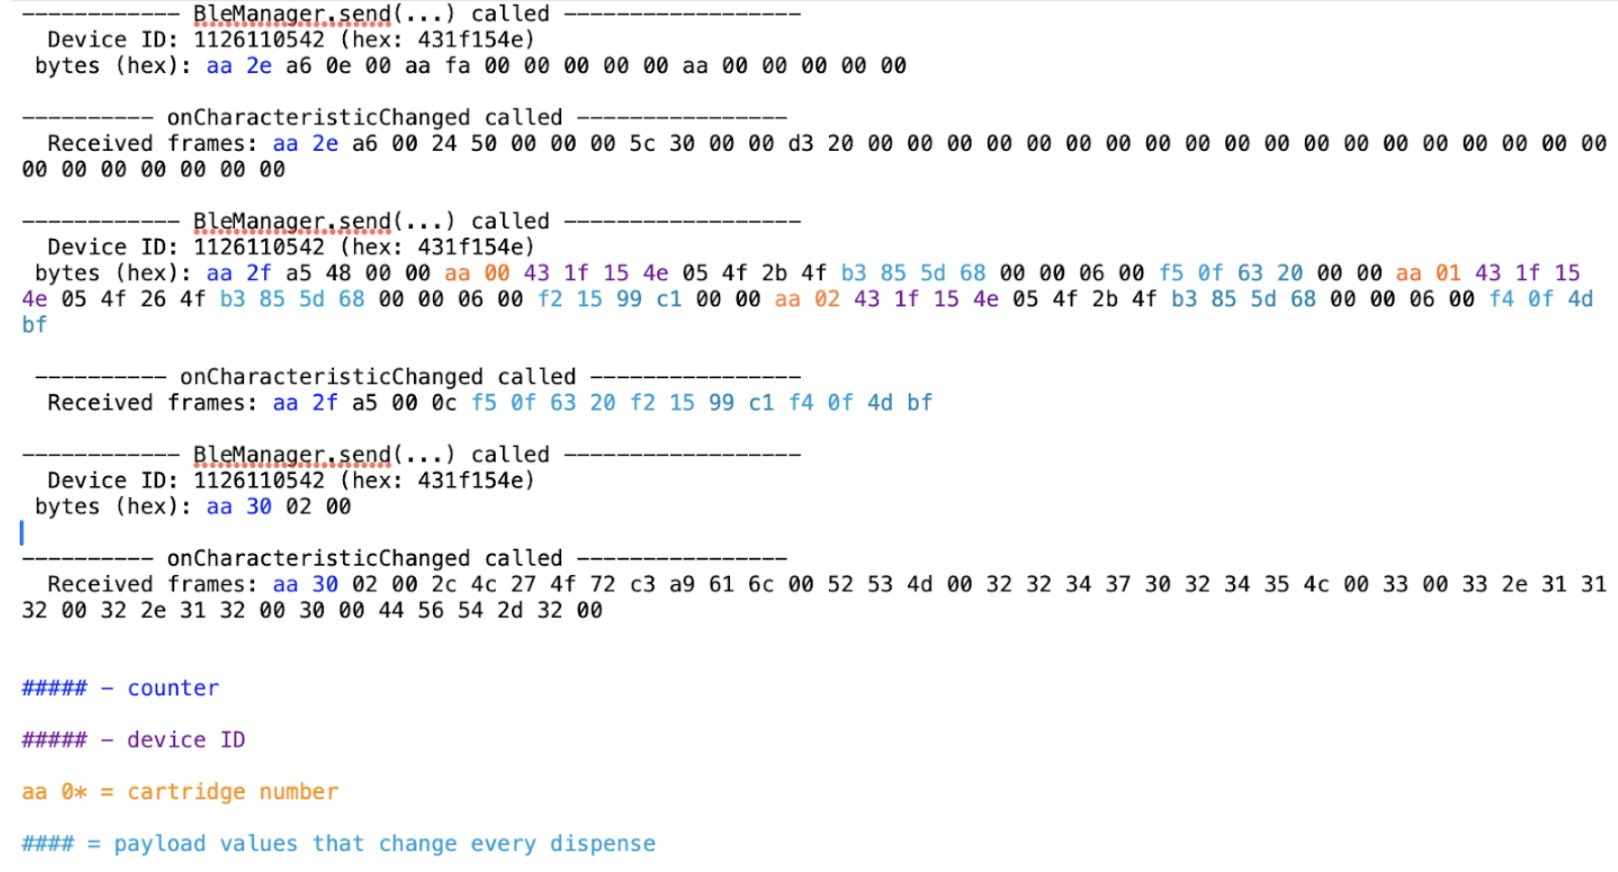
\includegraphics[width=0.7\linewidth]{payload4}
	\caption{Payload Four from dispenseFor(...) Hook}
	\label{fig:payload4}
\end{figure}

Using the cartridge data as a reference for what might appear in the larger payload, and knowing that volume is one of the most critical aspects of a dispense, I investigated whether the volume could be located within the payload. Because the volume changes between sends for the cartridges involved in dispensing, it was logical that the corresponding data would be part of the bytes that vary after each dispense. During testing, I noticed that when dispensing from only one cartridge, just two bytes would change within one of the four-byte sequences, while the remaining bytes stayed constant across dispenses. With a strong hypothesis about which bytes were significant, the next step was to test various ways these bytes could represent the volume information.

Identifying the correct data took several attempts. One significant obstacle was that, initially, I focused on locating the dispense volume itself, rather than recognizing that the volume appeared as the current total volume within each cartridge. With the realization that I should be looking for information in the cartridge data, representing the total volume per cartridge, and recalled that Android systems generally encode data in little-endian, the discovery became much clearer. Figure \ref{fig:payload5} illustrates the calculation of the volume derived from the payload. These calculations clearly line up with the 'Volume' numbers in Table \ref{tab:cartridgedata}
% TODO: \usepackage{graphicx} required
\begin{figure}[H]
	\centering
	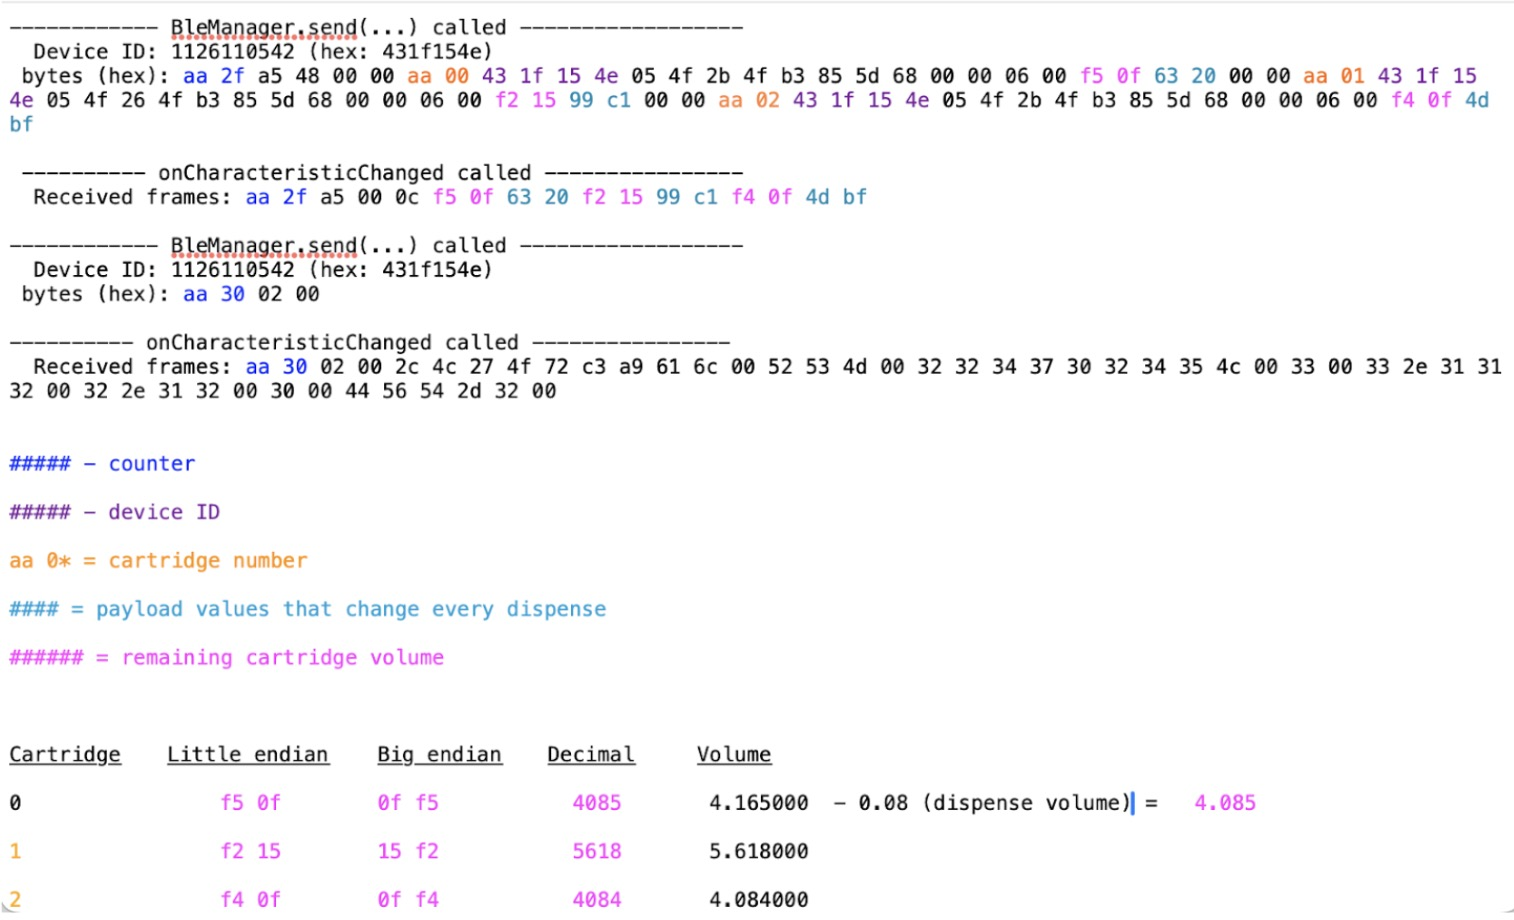
\includegraphics[width=0.7\linewidth]{payload5}
	\caption{Payload Five from the dispenseFor(...) Hook}
	\label{fig:payload5}
\end{figure}

After decoding the volume, there remained only one four-byte sequence and one two-byte sequence whose purposes were still unknown. To identify these, I revisited the cartridge information for additional clues. One recurring element in the cartridge data was information related to dates. Based on that insight, I experimented with reversing various combinations of bytes into big-endian format and using Python to convert these values into UTC datetime stamps. Ultimately, the full four-byte sequence before 00 00 06 was found to translate to the current print time.

% TODO: \usepackage{graphicx} required
\begin{figure}[H]
	\centering
	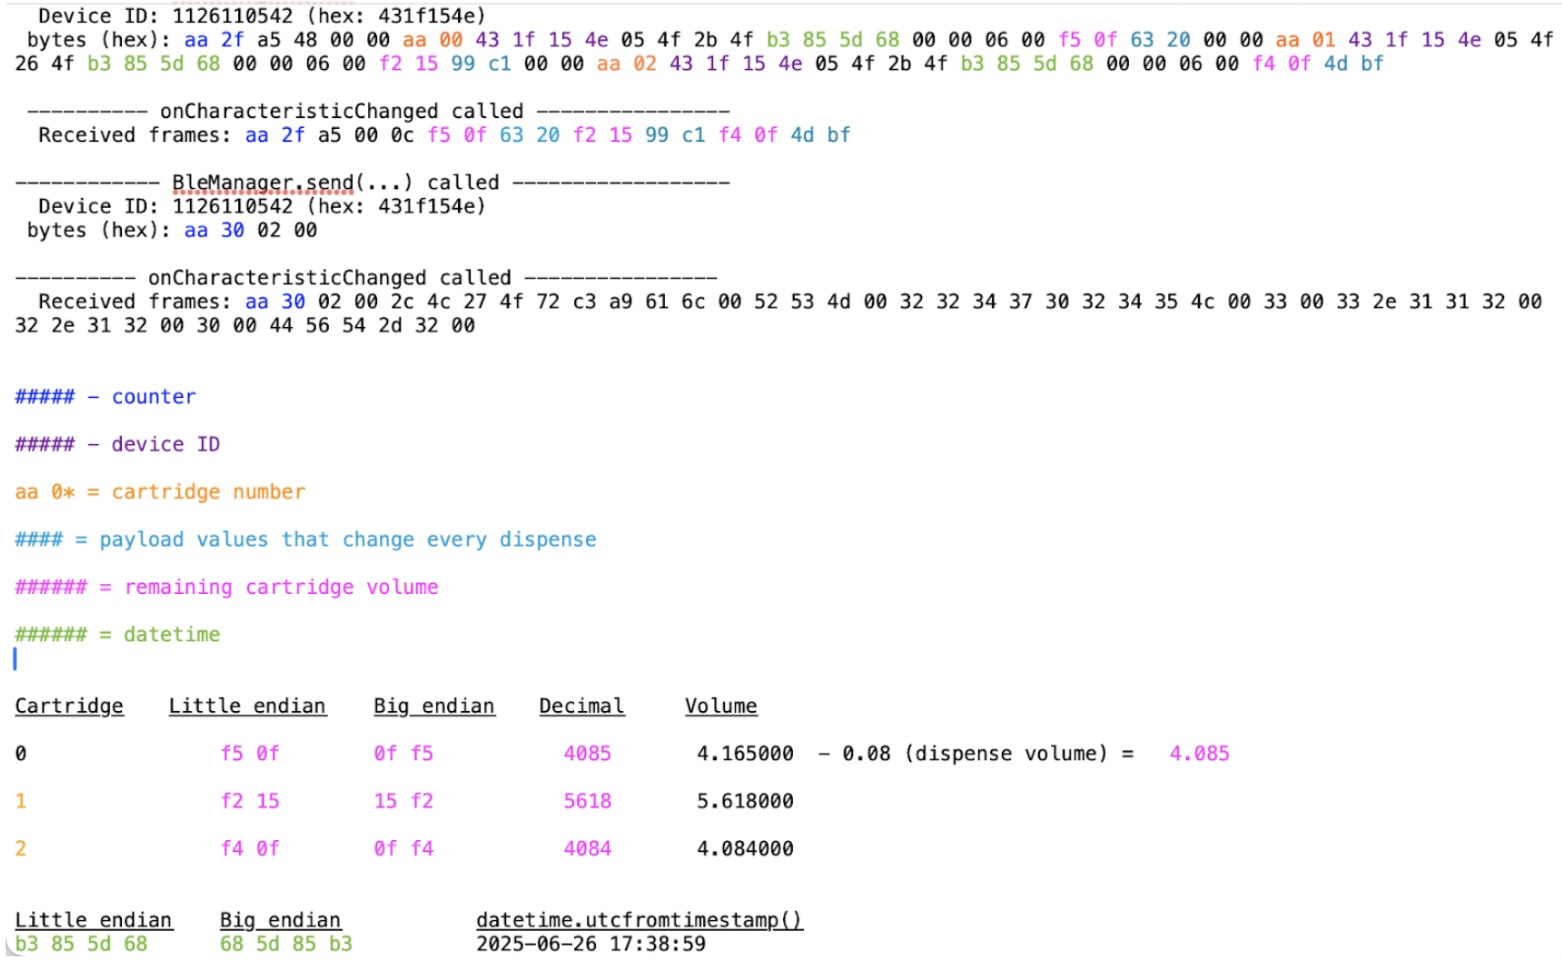
\includegraphics[width=0.7\linewidth]{payload6}
	\caption{Payload Six from the dispenseFor(...) Hook}
	\label{fig:payload6}
\end{figure}

With this understanding transmission over Bluetooth, it is feasible that if a third party application can be connected to the printer it could replicate these packets of data ad communicate with the device. My approach will be to inject code into the native application to modify its behavior.

Despite this shift in strategy, all the insights from analyzing the payloads remain valuable, as they help clarify the types of information the device expects to receive. This data has been documented for possible future use in crafting spoofed payloads. Figure \ref{fig:bigpayload} shows one of my comprehensive tests analyzing the byte payload from a pink dispense.
% TODO: \usepackage{graphicx} required
\begin{figure}[H]
	\centering
	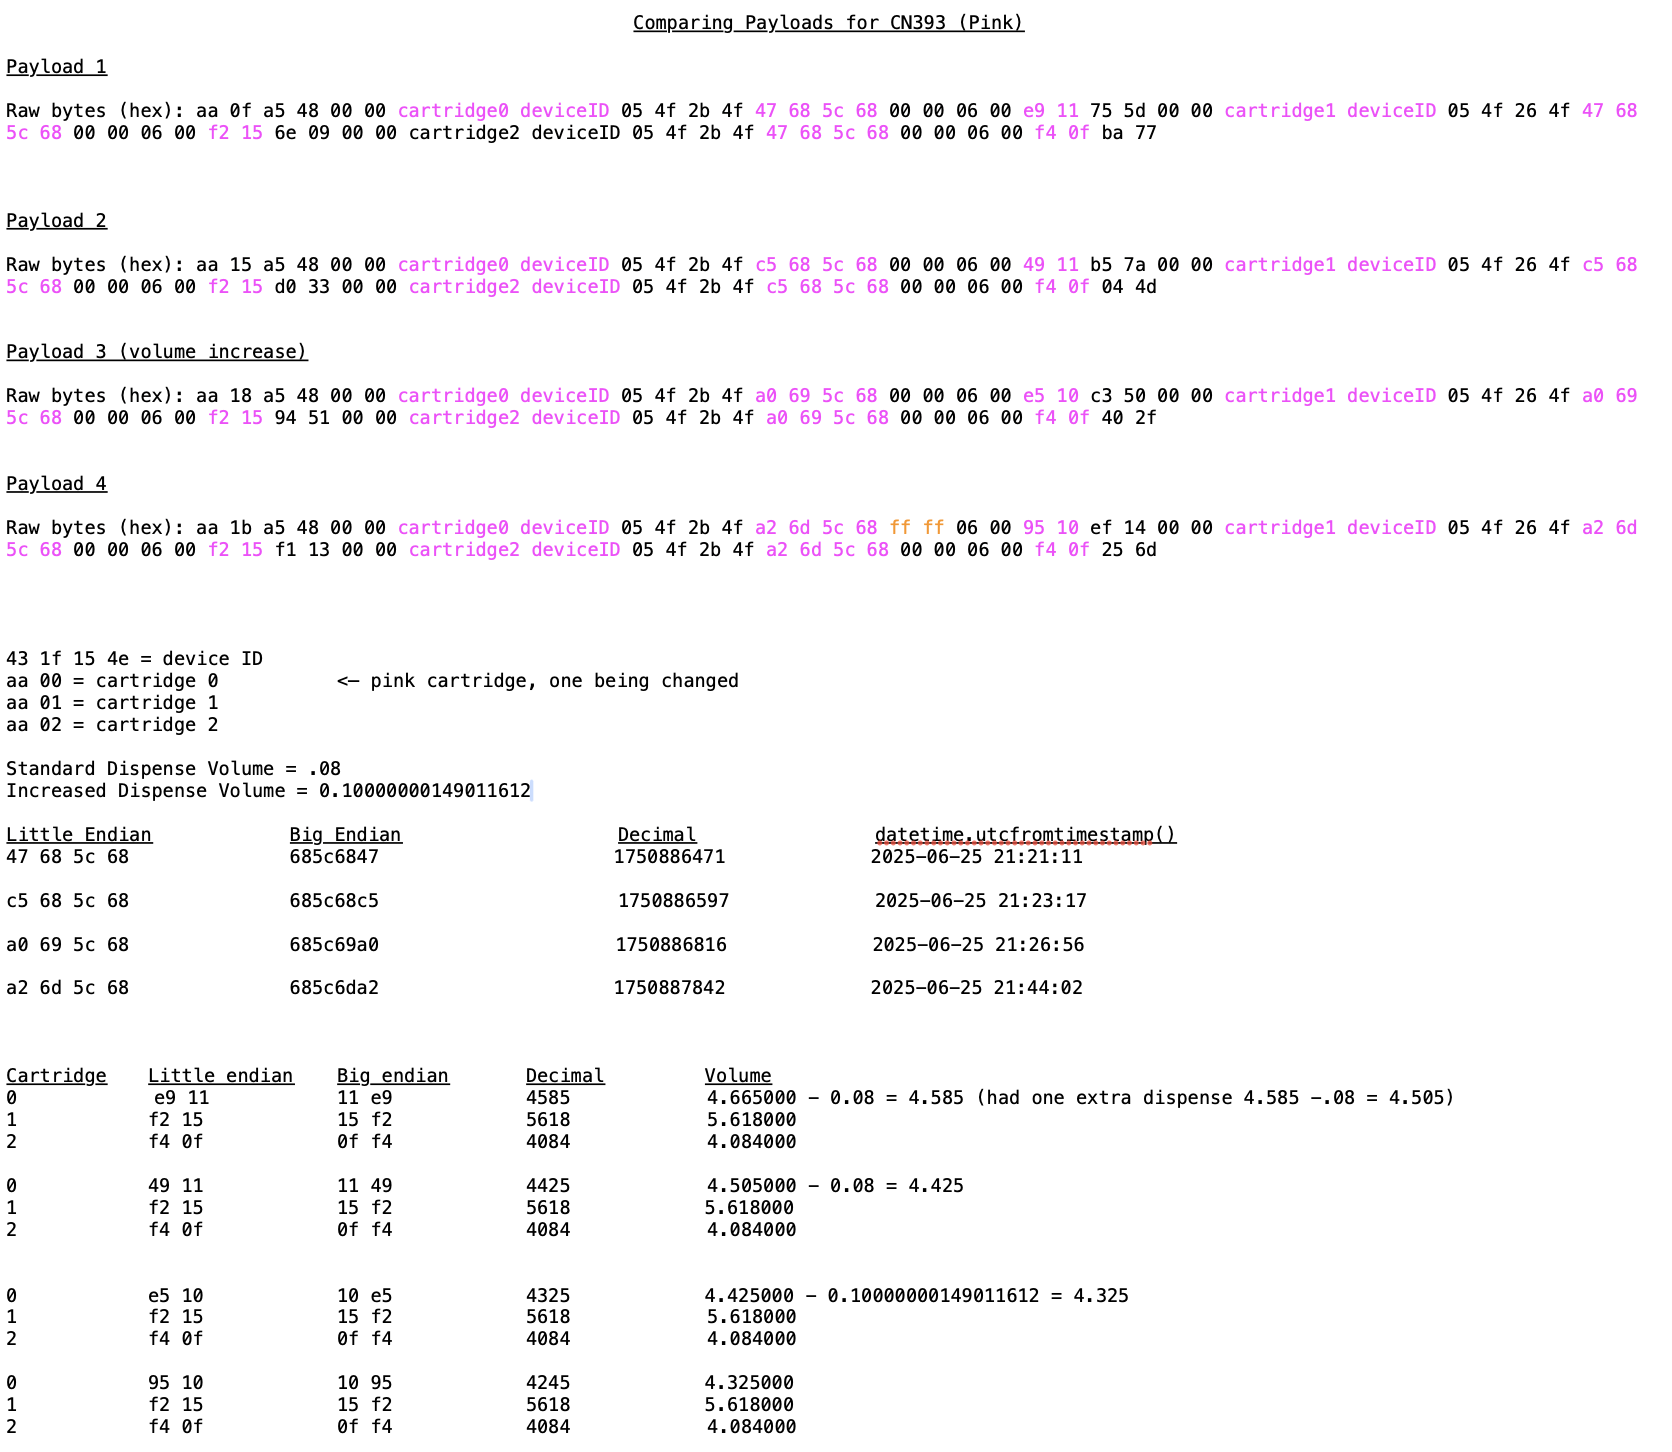
\includegraphics[scale=.3]{bigpayload}
	\caption{Multiple Payload Analysis}
	\label{fig:bigpayload}
\end{figure}


\section{Executing the Dispense}
With the comprehensive data gathered from earlier experiments, I set out to modify the color parameters and initiate a dispense. I once again used Frida’s straightforward Java method hooks, but in this iteration I directly manipulated the input variables of the \texttt{dispenseFor()} function. For clarity, the method signature is:
\begin{verbatim}
beamLipsController.dispenseFor(
    beamLipsDeviceId,
    colorUniverse,
    Color.red(color),
    Color.green(color),
    Color.blue(color),
    floatValue,
    intValue
);
\end{verbatim}
This function receives the cartridge universe identifier, the red, green, and blue components of the selected shade, the volume to dispense, and the dose count. My objective is to demonstrate the capacity to override these values at runtime. To achieve this, I redirected a dispense request originally set to light pink so that it produced a light brown output instead. Figure \ref{fig:environmentsetup} depicts the test arrangement, highlighting device connections and the sequence of operations.

% TODO: \usepackage{graphicx} required
\begin{figure}[H]
	\centering
	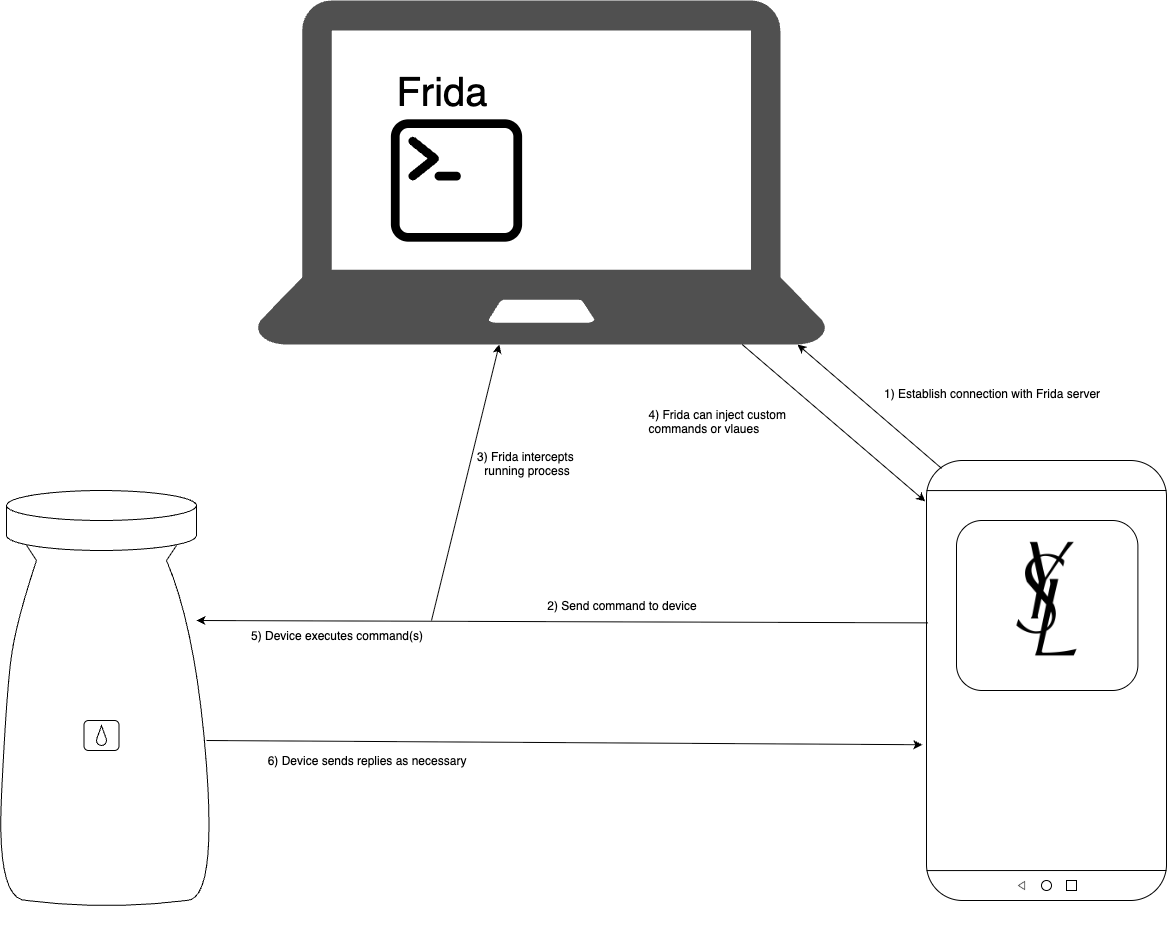
\includegraphics[width=0.7\linewidth]{environmentsetup}
	\caption{Dispense Environment Setup}
	\label{fig:environmentsetup}
\end{figure}

The Frida script follows the same pattern as previous hooks. First, I capture and log each incoming parameter to verify the original settings. I then replace the RGB values with those corresponding to the CN24 light brown shade, which are 200, 114, and 92 based on an earlier hook session. Finally, I invoke the original method with the modified values. The full script is presented below:
\begin{lstlisting}[language=JavaScript, breaklines=true]
Java.perform(function () {
    var BeamLipsController = Java.use("com.vinsol.loreal.PersoLips.utils.BeamLipsController");
    var overload = BeamLipsController.dispenseFor.overload(
        'int',
        'java.lang.String',
        'int',
        'int',
        'int',
        'float',
        'int'
    );
    
    overload.implementation = function(deviceId, colorUniverse, red, green, blue, volume, dose) {
        console.log("\n=== dispenseFor(...) called ===");
        console.log("Device ID: " + deviceId);
        console.log("Color Universe: " + colorUniverse);
        console.log("Original Red: " + red);
        console.log("Original green: " + green);
        console.log("Original Blue: " + blue);
        console.log("Original volume: " + volume);
        console.log("Original dose: " + dose);
        
        console.log("---------------------- Altering Color Values to print CN24 -------------------------");
        
        red = 200;
        green = 114;
        blue = 92;
        
        console.log("Modified Red: " + red);
        console.log("Modified Green: " + green);
        console.log("Modified Blue: " + blue);
        
        return overload.call(
            this,
            deviceId,
            colorUniverse,
            red,
            green,
            blue,
            volume,
            dose
        );
    };
    
    console.log("*** Hooked correct overload of dispenseFor in BeamLipsController ***");
});
\end{lstlisting}
The result was incredibly exciting. As shown in Figure \ref{fig:dispenseprint}, the device produced a light brown swatch even though the app remained set to light pink. However, the original light pink also appeared alongside the brown, despite only a single invocation of the modified \texttt{dispenseFor()} call. Furthermore, the final shade reported was CN63—a brown-pink hybrid that does not exist on the official color wheel (see Figure \ref{fig:cn63}).
% TODO: \usepackage{graphicx} required
\begin{figure}[H]
	\centering
	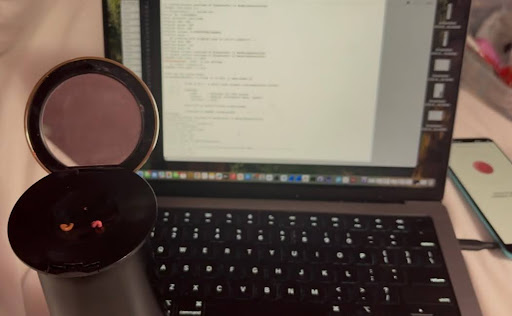
\includegraphics[scale=.7]{dispenseprint}
	\caption{Picture of Altered Dispense Output}
	\label{fig:dispenseprint}
\end{figure}
% TODO: \usepackage{graphicx} required
\begin{figure}[H]
	\centering
	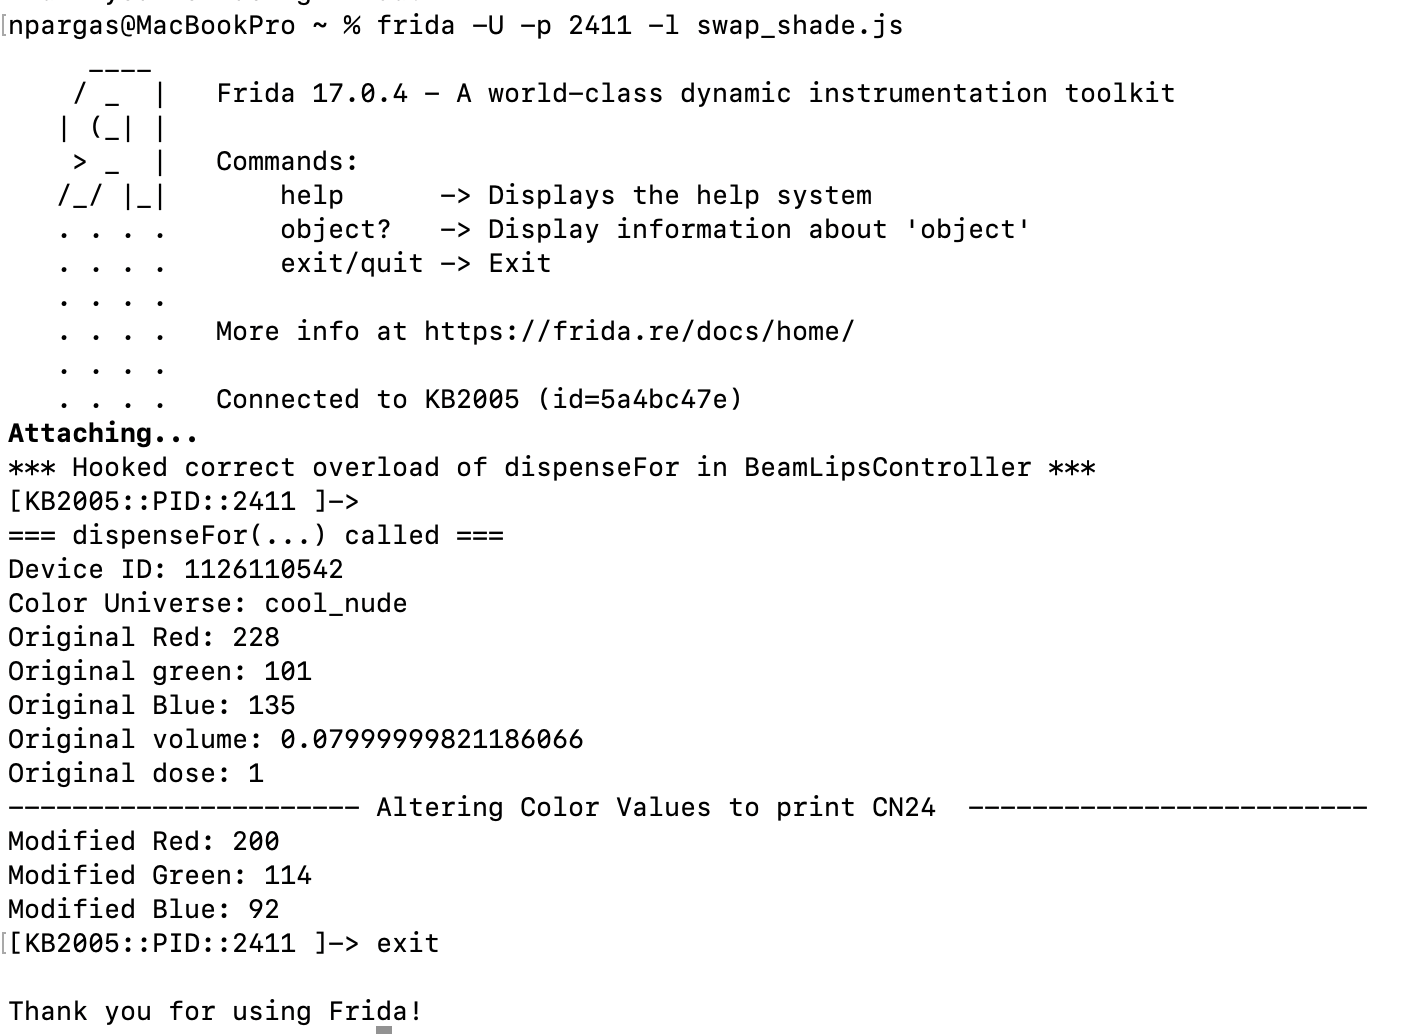
\includegraphics[scale=.15]{swapshadefrida}
	\caption{Frida Console Logs During Altered Dispense}
	\label{fig:swapshadefrida}
\end{figure}

% TODO: \usepackage{graphicx} required
\begin{figure}[H]
	\centering
	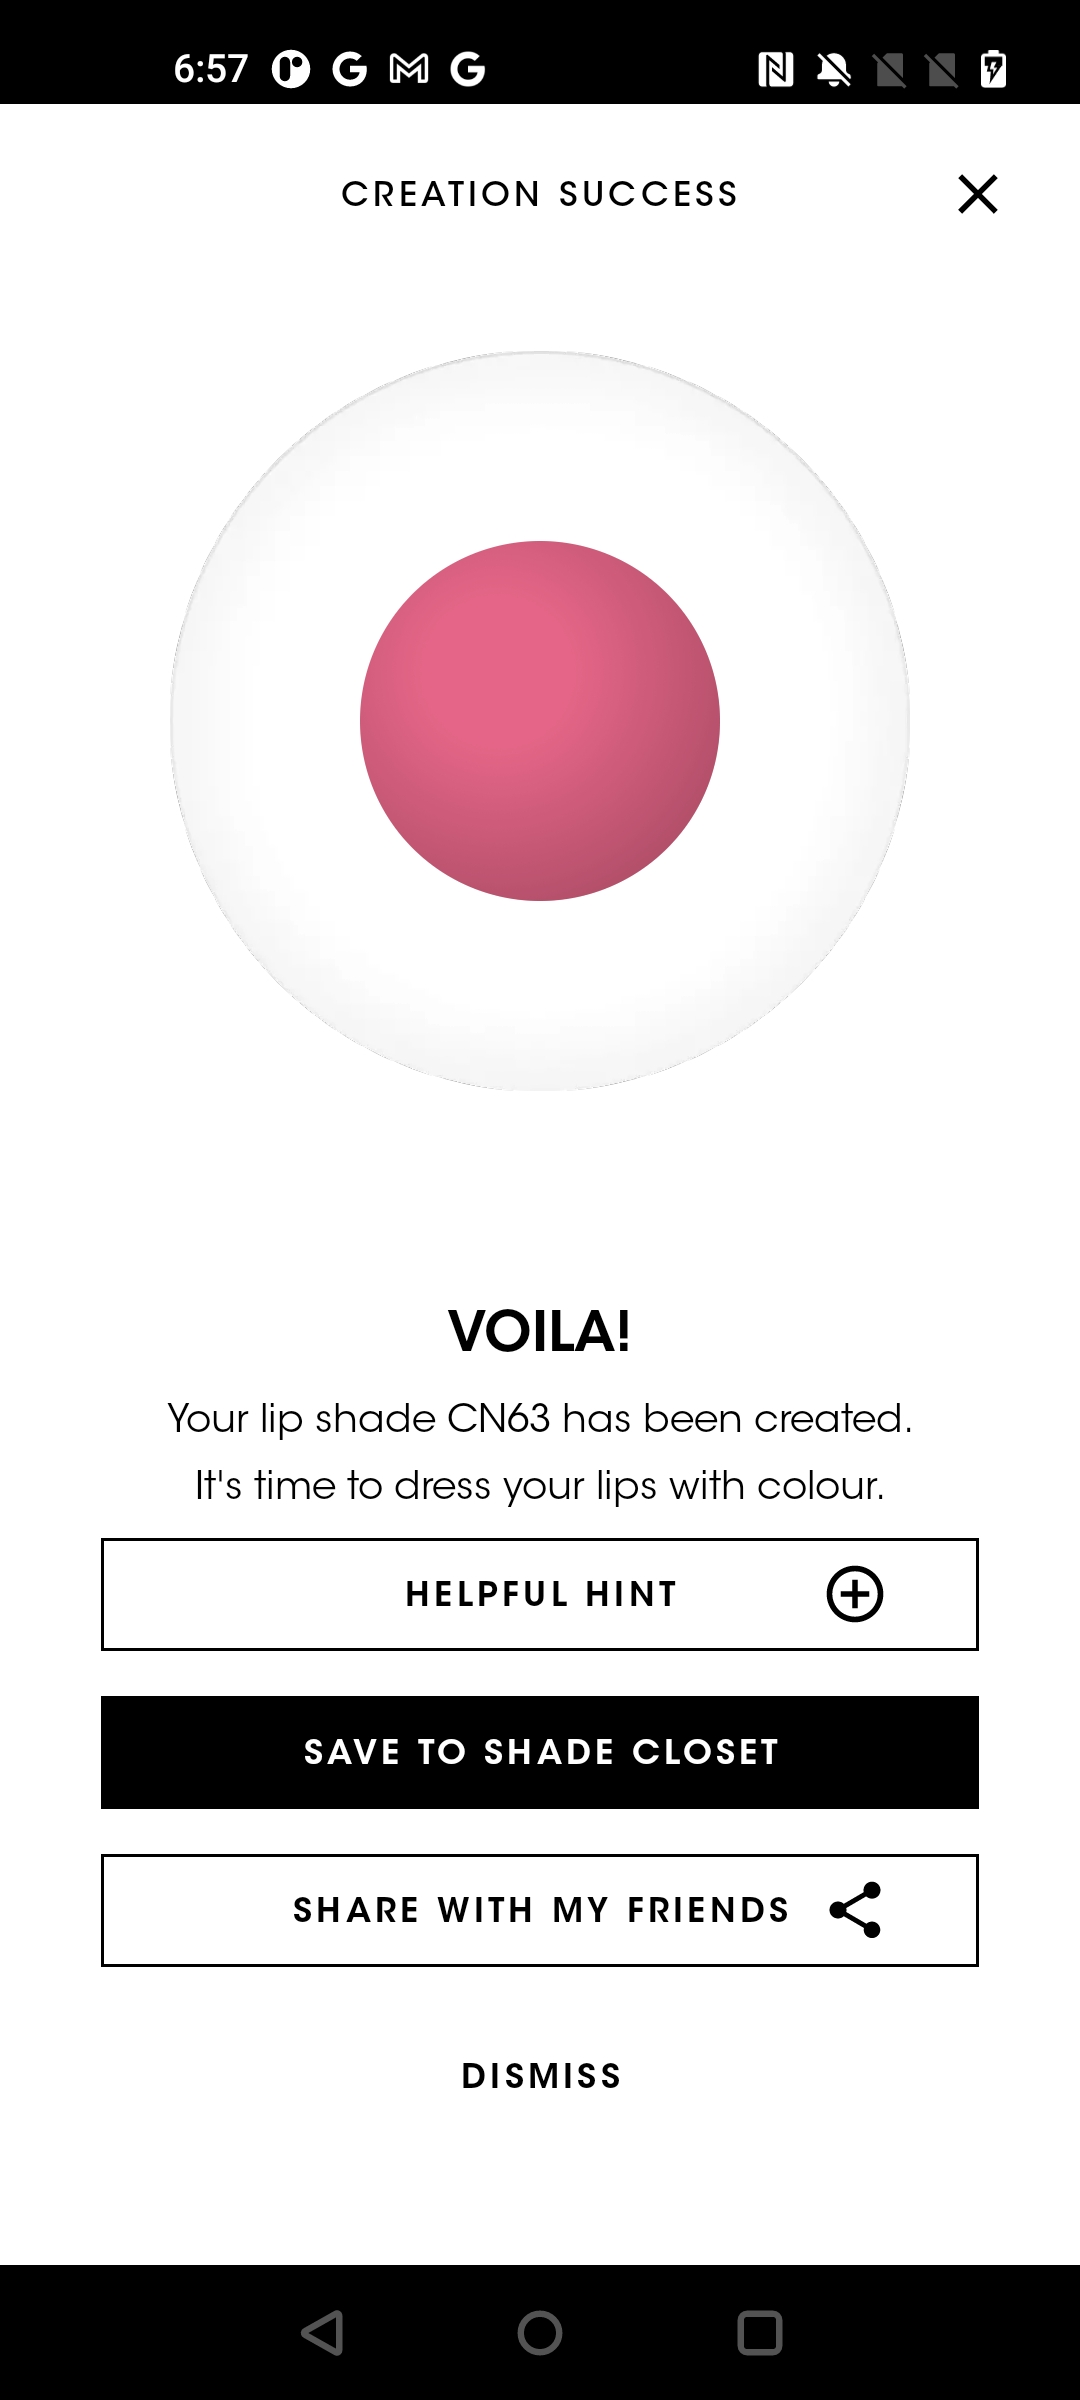
\includegraphics[scale=.15]{cn63}
	\caption{cn63 Screen Following Altered Dispense}
	\label{fig:cn63}
\end{figure}

These findings indicate that additional processing occurs after the RGB parameters are accepted. Possible explanations include internal blending algorithms, use of cached color values, or fallback logic within the application or firmware on the printer itself. To uncover the precise source of these effects, I could trace subsequent method calls and capture post-dispense data packets in future experiments

